% Chapter 2

\chapter{Spanish intonational phonology} % Chapter title

\label{ch:2}

As indicated in \chapref{ch:1}, the proliferation of sentence or \ac{TCU} level meanings as listed in Tables~\ref{tab:intonationalcategoriesPRIETOsmall} and~\ref{tab:intonationalcategoriesPRIETO} has turned \ac{SpToBI} into a system for the notation of nuclear configurations. This chapter tries to understand this as the result of an attempt to go beyond delimitative views on prosody (\sectref{ch:2.2}) and take distinctive functions of intonation on the level of entire dialogical turns seriously (\sectref{ch:2.3}). Yet it also argues that this requires us to have a theory of the kinds of dialogical meanings intonation can distinguish between, which is the subject of \chapref{ch:3}.


\section{Autosegmental-Metrical theory and Sp\_ToBI}
\label{ch:2.1}

The \ac{AM} theory of intonational phonology is the basis for the series of \ac{ToBI} transcription systems that has been developed since the last decade of the twentieth century. As \citet[42]{Ladd2008} lays out, it rests on four core assumptions, dating back to the seminal work by \citet{Pierrehumbert1980}: sequential tonal structure, distinction between pitch accent and stress, analysis of pitch accents in terms of Low L and High H level tones, and the analysis of pitch scaling in terms of an effect of iterated local changes.\footnote{In the following, the terms pitch and F$_0$ will be used interchangeably (see \cite[5]{Ladd2008} for an explanation).} Sequential tonal structure means that any pitch contour can be broken down into tones. Stretches between these tones are only seen as interpolations that are not phonologically distinctive.

The distinction between pitch accent and stress is an important part of what makes \ac{AM} theory autosegmental, because stress can be defined as the metrical prominence of a syllable at the word level \citep{Hyman2014,Buchholz.inprep}, whereas \acp{T} are au\-to\-no\-mous and lined up with either prominent positions or boundaries in a process called alignment. This gives rise to an \textit{intonation pattern} composed of \acp{T*}, \acp{T-} and \acp{Tpercent}. While sequential tonal structure and the distinction between pitch accents and stress have been generally adopted by research on Spanish intonation in the last three decades, the incorporation of a two-level distinction between H and L tones, combined with a view on pitch scaling in terms of iterated local changes, has been less consistent. \autoref{tab:intonationalcategoriesPRIETO} in \autoref{app:AppendixA} shows the prolific use of upstepped and downstepped tones in the description of Madrid Spanish intonation. The \acp{NI} with the indices c, d, e, h, and j make use of some sort of up- or downstep, indicated by exclamation marks in both vertical directions (! for `down', ¡ for `up'). As visible in \autoref{tab:intonationalcategoriesPRIETO}, both pitch accents and boundary tones are now made up of three tonal levels: L, H, and ¡H for pitch accents, and L, !H, and H for boundary tones. Only phrase accents have maintained the two-level distinction between L and H.

%Tracing the history of the diacritics for up- and downstep in  \ac{SpToBI} is actually a suitable way to get at many of today's unresolved issues in Spanish intonational phonology. Starting with \citet{BeckmanETAL.2002}, the question of how to deal with declarative sentences such as \textit{Le dieron el número del vuelo} `They gave her the flight number' in \autoref{fig:vuelo_BeckmanETAL} and \autoref{fig:vuelo_given_BeckmanETAL} led to concerns about how to represent the scaling differences between different prenuclear and nuclear peaks. 
%
%\begin{figure}
%	\centering
%	
%	\includegraphics[width=.95\linewidth]{gfx/figure_declarative_sentence_vuelo_BeckmanETAL.png}
%	\caption[Broad focus \textit{Le dieron el número del vuelo.}]{Declarative 
%		sentence \textit{Le dieron el número del vuelo.} `They gave her the flight 
%		number.' \citep[14]{BeckmanETAL.2002}. Response to \textit{¿Qué le dieron a 
%			María cuando fue al aeropuerto?} `What did
%		they give Maria when she went to the airport?'.}\label{fig:vuelo_BeckmanETAL}
%	
%	
%	\bigskip
%	\bigskip
%	
%	\includegraphics[width=.95\linewidth]{gfx/figure_declarative_sentence_vuelo_given_BeckmanETAL.PNG}
%	\caption[Final focus \textit{Le dieron el número del vuelo.}]{Final focus declarative \textit{Le dieron el número del vuelo.} `They gave her/him the flight number.' \citep[18]{BeckmanETAL.2002}. Response to \textit{¿Le dieron el número de vuelo o el número de asiento?} `Did
%		they give her/him the flight number or the seat number?'.}\label{fig:vuelo_given_BeckmanETAL}
%	
%\end{figure}
%
%One attempt was to use the idea of successively up- or downstepped sequences of tones to motivate these differences. Instead of formulating a universally applicable downtrend rule with iterated local changes in the tradition of \citet{Pierrehumbert1980}, the \ac{SpToBI} working group discussed if up- and downstep should be seen as a phonologically distinctive phenomenon that occurs in pragmatically marked utterances.\footnote{They thereby opted for a proposal by \citet{Ladd.1983} which intended to put forward a model that would reconcile the push for phonological generalizations by \citet{Pierrehumbert1980} with the need for phonetic detail in the establishment of feature-based natural classes in the sense of \citet[335--340]{ChomskyHalle.1968}.} Examples (\ref{ex:numerodelvuelo}a) and (\ref{ex:numerodelvuelo}b) show notational proposals for the scaling differences in \autoref{fig:vuelo_BeckmanETAL} and \autoref{fig:vuelo_given_BeckmanETAL}.\footnote{Note the differences to more recent notational conventions, namely the indication of an upstep at the beginning of a complex pitch accent ¡L$+$H* and the annotation of intermediate phrasing with a percent sign.}
%
%\noindent\begin{minipage}{\textwidth}
%\bigskip
%\begin{exe} % sets up the top-level example environment
%\ex\label{ex:numerodelvuelo} \citet[16,26]{BeckmanETAL.2002}
%\begin{xlist} % first embedding (alphabetical numbering)
%\ex  % example with running number
%\glll Le dieron el número del vuelo.\\
%~  | ~  | ~  | \\
%~ L*$+$H ~ L*$+$!H ~ L$+$!H* L\% \\
%
%\ex  % example with running number
%\glll Le dieron el número del vuelo.\\
%~  | ~  | ~  | \\
%~ L*$+$H ~ ¡L$+$H* H\% L$+$H* L\% \\
%
%
%\ex  % example with running number
%\glll Le dieron el número del vuelo.\\
%~  | ~  | ~  | \\
%~ L$+$H* ~ L$+$H* H$-$ L$+$H* L\% \\
%\end{xlist} % end first embedding
%\end{exe} % end example environment
%\bigskip
%\end{minipage}
%
%\citet[110--112]{Hualde.2002} reinterpreted the differences captured in 
%(\ref{ex:numerodelvuelo}) as an effect of the division between \textit{new} 
%and \textit{given} information. Together with \textit{focus-background 
%structure} and \textit{topic-comment structure}, these dichotomies form the 
%terminological basis for \ac{IS} as summarized by 
%\citet{KrifkaMusan.2012}. For the notation of Spanish intonation in the 
%\ac{AM} framework, the \ac{IS} perspective introduced by 
%\citet{Hualde.2002} comes with a significant change in notation. Instead 
%of an upstep analysis as in (\ref{ex:numerodelvuelo}b), 
%\citep[269]{Hualde.2014} opted for an analysis as an intermediate high 
%phrase accent H$-$, as in (\ref{ex:numerodelvuelo}c) and \autoref{fig:mariana_miraba_given_HUALDE}.
%
%\begin{figure}
%	\centering
%	
%	\includegraphics[width=.95\linewidth]{gfx/figure_mariana_miraba_given.jpg}
%	\caption[Subject and verb given in \textit{Mariana miraba la luna.}]{Declarative with given subject and verb \textit{Mariana miraba$_{H\textnormal{-}}$ la luna.} `Mariana was looking at the moon.' \citep[269]{Hualde.2014}.}\label{fig:mariana_miraba_given_HUALDE}
%	
%\end{figure}
%
%%illustrated in \autoref{fig:narrow_focus_final} and \autoref{fig:mariana_miraba_given_HUALDE}. 
%
%A visual comparison between \autoref{fig:vuelo_BeckmanETAL} and \autoref{fig:vuelo_given_BeckmanETAL} illustrates the implication of Hualde's proposal. Whereas the scaling of the second rising accent in \autoref{fig:vuelo_BeckmanETAL} is lower than the first, the scaling of the second rising accent in \autoref{fig:vuelo_given_BeckmanETAL} is higher. At the cost of this additional assumption, Hualde's proposal "freed up" the ¡ and the ! diacritics in \ac{SpToBI}, which have since been used to enrich the amount of tonal levels available in the inventories for pitch accents and boundary tones. 

 
Yet the complex system of pitch accents that arises from these additional tonal levels and their different alignments is mostly found within nuclear configurations. For prenuclear pitch accents, rises from L to H are the norm, with the main debate concerning alignment. \citet{HualdePrieto2015} state that prenuclear peaks in Spanish rising accents can be aligned either with the tonic or the posttonic syllable of polysyllabic words that do not bear lexical stress on the ultimate syllable and leave open the question whether they are in complementary distribution, which is a disputed point in the literature. \citet[106]{Hualde.2002} presents rising accents in Spanish as underspecified with respect to tonal alignment (\ref{ex:risingaccentshualde}). As in \autoref{tab:intonationalcategoriesGABRIEL}, the proximity to phrase accents and boundary tones can then determine the early or late alignment of the H tone. \citet{FacePrieto.2007}, on the other hand, argue that Madrid Spanish has three phonologically distinct rising accents, L+H*, L+<H*, and L*+H, which are determined by an interplay between two dichotomies: declarative vs. interrogative, and broad vs. narrow focus.

\begin{exe}
\ex\label{ex:risingaccentshualde} Phonological representation of rising accents in Spanish \citep[106]{Hualde.2002}\\
~\hspace*{2em} * \\
%\begin{xlist}
\glll [..... ($\sigma$) .....] word\\
~  | ~ ~ \\
~ L$+$H \\
%\end{xlist}
\end{exe}

%\begin{figure}
%\centering
%
%\includegraphics[width=.95\linewidth]{gfx/figure_narrow_focus_statement_initial.jpg}
%\caption[Initial focus \textit{Bebe la limonada.}]{Narrow initial focus declarative \textit{Bebe la limonada.} `(She) drinks the lemonade.' \citep[369]{HualdePrieto2015}.}\label{fig:narrow_focus_initial}
%
%\bigskip
%
%
%\includegraphics[width=.95\linewidth]{gfx/figure_narrow_focus_statement_final.jpg}
%\caption[Verb given in \textit{Bebe la limonada.}]{Declarative with given verb \textit{Bebe la limonada.} `(She) drinks the lemonade.' \citep[370]{HualdePrieto2015}.}\label{fig:narrow_focus_final}
%
%\bigskip
%
%\end{figure}




The problem of choosing between three different labels for prenuclear rising pitch accents or a single label with different realizations according to the presence or absence of an intervening phrase accent hints at a deeper problem that affects the entire description of Spanish intonation. Whereas the analysis of phonological phrasing relies on functional dichotomies such as \textit{focus} and \textit{background} or \textit{given} and \textit{new} information, which divide sentences into domains of \ac{IS} \citep{KrifkaMusan.2012} and are therefore prone to be expressed prosodically by accents with \textit{delimitative} functions (in the sense of \cite[29]{Trubeckoj1939}), the paradigmatic choice between different pitch accents, phrase accents, and boundary tones has been related to nuclear configurations that encode obviousness, exclamation, insistence and other meanings. This dichotomy is key in understanding the different approaches to prosody that have guided the literature on intonation. Showing its importance will be the goal of the rest of this chapter, which is structured accordingly.



\section{Delimitation}
\label{ch:2.2}

%##### H$-$ associated to the right edge of an IP in $+$obvious $+$agree, 
%but 
%pushed leftwards by nuclear pitch accent???

Delimitative approaches to prosody have to deal with several layers of 
complexity. And as will become clear, this complexity arises in part because of 
paradigmatic relations between types of boundaries and syntagmatic 
relations between pitch accents and boundary tones that compete for 
alignment with the segmental string. Delimitative approaches are usually considered to 
establish a relation between syntactic and phonological boundaries, 
usually in the form of some kind of correspondence or \textit{mapping} 
between syntactic constituency, \ac{IS}, and prosodic 
constituency (\sectref{ch:2.2.1}).\footnote{Note that 
the term mapping is sometimes also used for \textit{tone mapping rules}, 
which serve to calculate the phonetic value of tones in sequences relative 
to the preceding ones \citep[105]{Fery.2017}. We restrict the term to the 
syntax-prosody interface.} They then have to give accounts for the tonal 
categories that express the boundaries of these prosodic constituents 
(\sectref{ch:2.2.2}). Finally, they need to decide whether they see pitch 
scaling and alignment as relevant for the delimitation of prosodic constituents (\sectref{ch:2.2.3}).

\subsection{Mapping}\label{ch:2.2.1}\largerpage[2]

\citet[63]{Fery.2017} distinguishes between what we could broadly call a 
\textit{one-edge} and a \textit{two-edge} approach. Without using the terms 
\textit{one-edge}/\textit{two-edge approach} herself, \citet{Fery.2017} groups 
\textit{relation-based}, \textit{edge-based}, and \textit{alignment} approaches 
as those which map pre-existing syntactic constituents at one edge to 
prosodic constituents, whereas \textit{containment} and \textit{match} 
strategies map syntactic constituents to prosodic constituents at two 
points in the speech chain. 

One-edge approaches allow for mismatches between syntactic and prosodic constituents and therefore lend themselves to explaining cases in which a local prosodic marking is supposedly ambiguous between a local and a broader (possibly sentence-level) interpretation. The classic example for such an ambiguity is sentence-final stress, which in Spanish and other Romance and Germanic languages has been found to be ambiguous between narrow focus on the final constituent and broad focus on the entire sentence \citep[36]{Gabriel2007}. Example (\ref{ex:focuspercolation}) shows a broad focus declarative sentence in which the focus feature F “percolates” from the prominent last word to the sentence as a whole.{\interfootnotelinepenalty=10000\footnote{Focus “percolation” refers to the idea in generative syntax that the focus feature F passes the maximal projection of the accented terminal node and attaches to higher levels of syntactic structure.}}

\begin{exe}
\ex\label{ex:focuspercolation} Based on \citet[65]{Gabriel2007} \\
 María compra el diario en $_{F}$[el KIOSco.]$_{F}$~$\longmapsto$\\
 $_{F}$[María compra el diario en el KIOSco.]$_{F}$ 
\glt `Maria buys the newspaper at the kiosk.’
\end{exe}

%(\ref{ex:RelativeProminenceRuleNESPORVOGEL})
%(\ref{ex:phiphraserestructuringNESPORVOGEL})

An example of a relational rule would be the \textit{Relative Prominence} rule, which assigns prominence to either the right or the left edge of a $\phi$-phrase depending on the direction of syntactic branching in that language. Prominence, in turn, would then be a cue that helps us delimit $\phi$-phrases. According to the original approach by \citet{Nespor2007}, the $\phi$-phrase is aligned with a syntactic phrase dominated by one syntactic head. A leftmost head position implies rightward branching, which in turn would imply rightmost prominence in complex constituents. To allow for $\phi$-phrases that include more than one syntactic head, this approach allows for optional $\phi$-phrase restructuring, thereby 
licensing (\ref{ex:restructuringexamplesFERY}a-b), but not 
(\ref{ex:restructuringexamplesFERY}c).\footnote{Note that a proposal for rhythm-based restructuring by \citet{Ghini.1993} still obeys strong syntactic boundaries as in (\ref{ex:restructuringexamplesFERY}c).}

%\noindent\begin{minipage}{\textwidth}
%\bigskip
%\begin{exe}
%\ex\label{ex:RelativeProminenceRuleNESPORVOGEL} Relative Prominence \citet[168]{Nespor2007}\\
%\begin{spacing}{0.5}
%In languages whose syntactic trees are right branching, the rightmost node of a $\phi$-phrase is labelled s (for strong); in languages whose syntactic trees are left branching, the leftmost node of a $\phi$-phrase is labelled s. All other nodes are labelled w (for weak).\\
%\end{spacing}
%%\end{xlist}
%\end{exe}
%\end{minipage}

%\noindent\begin{minipage}{\textwidth}
%\bigskip
%\begin{exe}
%\ex\label{ex:phiphraserestructuringNESPORVOGEL} Optional $\phi$-phrase restructuring according to \citet{Nespor2007} as illustrated by \citet[67]{Fery.2017}\\
%\begin{spacing}{0.5}
%A nonbranching $\phi$-phrase that is the first complement of X on its
%recursive side is joined into the $\phi$-phrase that contains X.\\
%\gll ~.....X ~...... ~ ~......X...... \\
%(~~~~~~~)$_\phi$ (~~~~~)$_\phi$ $\longmapsto$ 
%(~~~~~~~~~~~~)$_\phi$ \\
%\end{spacing}
%%\end{xlist}
%\end{exe}
%\end{minipage}

\begin{exe}
\ex\label{ex:restructuringexamplesFERY} Optional $\phi$-phrase restructuring according to \citet{Nespor2007} as illustrated by \citet[67]{Fery.2017}
\begin{xlist}
\ex Italian\\
(I~caribù)$_\phi$~(nani)$_\phi$~(sono~estinti)$_\phi$~$\longmapsto$ (I~caribù~nani)$_\phi$~(sono~estinti)$_\phi$ 
\glt  `Dwarf~caribous~are~extinct.'
\ex 
(Darò)$_\phi$~(un~libro)$_\phi$~(a~Gianni)$_\phi$~$\longmapsto$ (Darò~un~libro)$_\phi$~(a~Gianni)$_\phi$ 
\glt `I'll~give~a~book~to~Gianni.' 
\ex 
(Papà)$_\phi$~(mangia)$_\phi$~$\not\longmapsto$ *(Papà~mangia)$_\phi$ 
\glt`Dad~is~eating.'
\end{xlist}
%\end{xlist}
\end{exe}

The crucial problem for the current discussion is the incompatibility of such a relational approach with a prosodic form as in \autoref{fig:mariana_miraba_given_HUALDE} from \citet[269]{Hualde.2014}, which shows the typical intonation of a response to \textit{¿Qué miraba Mariana?} `What was Mariana looking at?'.\footnote{Given that most publications are not open-access, intonation research is faced with the problem of how to cite pitch contours. Stylization will be used for pitch contours from commercial publications throughout this introduction.} A rule that prohibits restructuring of (S)(V) to (SV) as in (\ref{ex:restructuringexamplesFERY}c) does not allow for restructuring of (S)(V)(O) to (SV)(O) as in (\ref{ex:restructuringexamplesMARIANA}) either.\largerpage[-1]


\begin{figure}
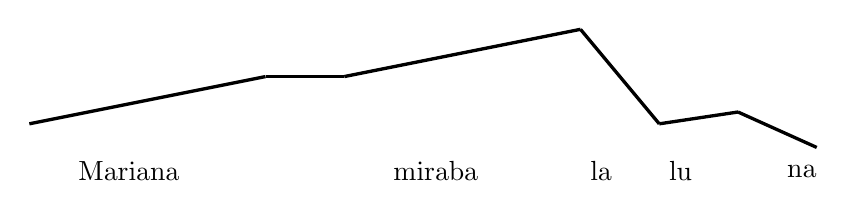
\begin{tikzpicture}[yscale = 0.6]
	\draw [very thick] (0,0.5) -- (3,1.5);
	\draw [very thick] (3,1.5) -- (4,1.5);
	\draw [very thick] (4,1.5) -- (7,2.5);
	\draw [very thick] (7,2.5) -- (8,0.5);
	\draw [very thick] (8,0.5) -- (9,0.75);
	\draw [very thick] (9,0.75) -- (10,0);
				
	\node[anchor=west] at (0.5,-0.5) {Mariana};
	\node[anchor=west] at (4.5,-0.5) {miraba};
	\node[anchor=west] at (7,-0.5) {la};
	\node[anchor=west] at (8,-0.5) {lu};
	\node[anchor=west] at (9.5,-0.5) {na};
\end{tikzpicture}
\caption{Declarative with given subject and verb \textit{Mariana miraba$_{H\textnormal{-}}$ la luna.} `Mariana was looking at the moon.' \citep[269]{Hualde.2014}.\label{fig:mariana_miraba_given_HUALDE}}
\end{figure}

%\begin{figure}
%	\centering
%	
%	\includegraphics[width=.95\linewidth]{gfx/figure_mariana_miraba_given.jpg}
%	\caption[Subject and verb given in \textit{Mariana miraba la luna.}]{Declarative with given subject and verb \textit{Mariana miraba$_{H\textnormal{-}}$ la luna.} `Mariana was looking at the moon.' \citep[269]{Hualde.2014}.}\label{fig:mariana_miraba_given_HUALDE}
%	
%\end{figure}


\begin{exe}
\ex\label{ex:restructuringexamplesMARIANA} 
(Mariana)$_\phi$~(miraba)$_\phi$~(la~luna)$_\phi$~$\not\longmapsto$ *(Mariana~miraba)$_\phi$~(la~luna)$_\phi$ 
\glt `Mariana~was~looking~at~the~moon.' 
\end{exe}

\textit{Edge-based} approaches \citep{Chen.1987,Chen.2000}, which allow for 
$\phi$-phrases to cross the boundaries of syntactic phrases by projecting 
$\phi$-phrases from maximal projections, still fall short of accounting 
for  \autoref{fig:mariana_miraba_given_HUALDE}. They allow for 
$\phi$-phrases that contain verbs and their complements, or even verbs and 
adjuncts, but external arguments seem to be problematic.\footnote{See 
\citet{KoopmanSportiche.1991} as well as 
\citet[75--80]{Gabriel_Mueller_Fischer.2018} for an account that generates 
subjects inside the \ac{VP} for $\theta$-role assignment and then moves 
them to an external position for further grammatical feature assignment 
and serialization of the surface word-order. Nevertheless, the visibility 
of syntactic movement to prosodic structure would pose a problem to any 
modular theory of grammar that takes a syntactic form as an input to 
prosodic structure, a mechanism upheld even in so-called 
\textit{try-and-filter approaches} which select between different syntactic 
forms on the basis of prosodic requirements \citep[872--873]{Buring.2013}.} All in all, the inviolable mapping rules presented so far seem 
descriptively inadequate if (SV)(O) is to be within the realm of 
possibilities.

%(\ref{ex:alignRL})
%(\ref{ex:wrapXP})
%(\ref{ex:stressXP}) 
%(\ref{ex:NonRec})

\ac{OT} based systems like the one in \citet{Truckenbrodt.1995} move past the 
simple \textit{one-edge}/\textit{two-edge} dichotomy in combining one-sided 
alignment constraints like \textsc{Align ($\phi$, R, L)} with two-sided matching constraints like 
\textsc{Wrap-XP}. They go even further in incorporating 
stress-assign\-ment mechanisms like \textsc{Stress-XP} 
and constraints on prosodic domination like \textsc{Nonrecursivity 
(NonRec)} into the list of constraints on 
$\phi$-phrasing, which together select an optimal candidate in sentences 
with two or more \acp{XP} as in (\ref{ex:OTlaotraamiga}). Most 
importantly, though, \ac{IS} categories such as \textit{focus} can be 
incorporated as a high-ranking constraint like \textsc{Stress Focus} 
(\ref{ex:stressfocus}) \citep[235]{Gabriel2007} that override other 
mapping requirements to give rise to marked prosodic structures as in 
(\ref{ex:OTlaotraamigaFOCUS}).
%
%\noindent\begin{minipage}{\textwidth}
%\bigskip
%\begin{exe}
%\begin{spacing}{0.5}
%\ex\label{ex:alignRL} \textsc{Align ($\phi$, R, L)} \citep[43]{Truckenbrodt.1995} \\
%\begin{xlist}
%\ex 
%\textsc{Align ($\phi$, R)}: Align the right edge of every XP with the right edge of a phonological phrase. \\
%\ex
%\textsc{Align ($\phi$, L)}: Align the left edge of every XP with the left edge of a phonological phrase. \\
%\end{xlist}
%\end{spacing}
%\end{exe}
%\end{minipage}
%
%\noindent\begin{minipage}{\textwidth}
%\bigskip
%\begin{exe}
%\begin{spacing}{0.5}
%\ex\label{ex:wrapXP} \textsc{Wrap-XP} \citep[81--82]{Truckenbrodt.1995} \\
%\medskip \\
%\textsc{Wrap-XP} $\leftrightarrow$ for every XP, XP a projection of a lexical category, there is a phonological phrase $\phi$, such that all terminal elements that are dominated by XP are also dominated by $\phi$.\\
%\end{spacing}
%\end{exe}
%\end{minipage}
%
%\noindent\begin{minipage}{\textwidth}
%\bigskip
%\begin{exe}
%\begin{spacing}{0.5}
%\ex\label{ex:stressXP} \textsc{Stress-XP} \citep[226]{Truckenbrodt.1995} \\
%\medskip \\
%Each lexically headed XP must contain a phrasal stress X$_\phi$. \\
%\end{spacing}
%\end{exe}
%\end{minipage}
%
%\noindent\begin{minipage}{\textwidth}
%\bigskip
%\begin{exe}
%\begin{spacing}{0.5}
%\ex\label{ex:NonRec} \textsc{NonRec} \citep{Selkirk.1995} \\
%\medskip \\
%\textsc{NonRec} $\leftrightarrow$ No C$^i$ dominates C$^j$, j=i \medskip\\
%No prosodic category C dominates another prosodic category of the same type, e.g. ``no $\phi$ dominates a $\phi$''.
%\end{spacing}
%\end{exe}
%\end{minipage}

\begin{exe}
\ex\label{ex:stressfocus} \textsc{Stress Focus (SF)} \citep[235]{Gabriel2007} \\
$_F$[X/XP]$_F$ is prosodically more prominent than [Y/YP].


\ex\label{ex:OTlaotraamiga} Based on \citet[230]{Truckenbrodt.1995} and \citet[77]{Fery.2017}\smallskip\\
\begin{tabular}{|rl||cccc|}
\hline
& [la.ˈo.tɾa]$_\omega$[a.ˈmi.ɣa]$_\omega$ & \small{\textsc{Wrap}} & \small{\textsc{Stress}} & \small{\textsc{Align}} & \small{\textsc{Non}}\\
& [mi.ˈɣa.βa]$_\omega$[la.ˈlu.na]$_\omega$ & \small{\textsc{XP}} & \small{\textsc{XP}} & \small{\textsc{($\phi$,R)}} & \small{\textsc{Rec}}\\
\hline\hline
\ding{43}~a. & [la.ˌo.tɾa.a.ˈmi.ɣa]$_\phi$ & \multirow{2}{*}{}  & \multirow{2}{*}{} & \multirow{2}{*}{} & \multirow{2}{*}{} \\
& [mi.ˌɾa.βa.la.ˈlu.na]$_\phi$ & & & &\\
\hline
b. & [la.ˌo.tɾa.a.ˈmi.ɣa & \multirow{2}{*}{} & \multirow{2}{*}{} & \multirow{2}{*}{} & \multirow{2}{*}{*}\\
& [mi.ˌɾa.βa.la.ˈlu.na]$_\phi$]$_\phi$ & & & &\\
\hline
c. & [la.ˌo.tɾa.a.ˈmi.ɣa]$_\phi$ & \multirow{2}{*}{*} & \multirow{2}{*}{} & \multirow{2}{*}{} & \multirow{2}{*}{}\\
& [mi.ˈɣa.βa]$_\phi$[la.ˈlu.na]$_\phi$ & & & &\\
\hline
d. & [la.ˌo.tɾa.a.ˌmi.ɣa & \multirow{2}{*}{*} & \multirow{2}{*}{*} & \multirow{2}{*}{*} & \\
& mi.ˌɾa.βa.la.ˈlu.na]$_\phi$& & & &\\
\hline
e. & [la.ˌo.tɾa.a.ˌmi.ɣa & \multirow{2}{*}{**} & \multirow{2}{*}{*} & \multirow{2}{*}{*} & \multirow{2}{*}{}\\
& mi.ˈɣa.βa]$_\phi$[la.ˈlu.na]$_\phi$ &  &  &  &\\
\hline
\end{tabular}


\ex\label{ex:OTlaotraamigaFOCUS}
\begin{tabular}[t]{|rl||ccccc|}
\hline
& $_F$[la.ˈo.tɾa]$_\omega$$_F$[a.ˈmi.ɣa]$_\omega$ & \multirow{2}{*}{\small{\textsc{SF}}} & \small{\textsc{Wrap}} & \small{\textsc{Str.}} & \small{\textsc{Al.}} & \small{\textsc{Non}} \\
& [mi.ˈɣa.βa]$_\omega$[la.ˈlu.na]$_\omega$ & &  \small{\textsc{XP}} & \small{\textsc{XP}} & \small{\textsc{($\phi$,R)}} & \small{\textsc{Rec}} \\
\hline\hline
\ding{43}~a. & [la.ˈo.tɾa [a.mi.ɣa & \multirow{2}{*}{} & \multirow{2}{*}{**} & \multirow{2}{*}{} & \multirow{2}{*}{*} & \multirow{2}{*}{*} \\
& mi.ɾa.βa.la.ˌlu.na]$_\phi$]$_\phi$ & & & & & \\
\hline
b. & [la.ˈo.tɾa]$_\phi$[a.ˌmi.ɣa & \multirow{2}{*}{*} & \multirow{2}{*}{\cellcolor[gray]{0.8}**} & \multirow{2}{*}{\cellcolor[gray]{0.8}} & \multirow{2}{*}{\cellcolor[gray]{0.8}*} & \multirow{2}{*}{\cellcolor[gray]{0.8}} \\
& mi.ˌɾa.βa.la.ˈlu.na]$_\phi$ & & \cellcolor[gray]{0.8} & \cellcolor[gray]{0.8} & \cellcolor[gray]{0.8} & \cellcolor[gray]{0.8} \\
\hline
c. & [la.ˈo.tɾa]$_\phi$[a.ˈmi.ɣa]$_\phi$ & \multirow{2}{*}{**} & \multirow{2}{*}{\cellcolor[gray]{0.8}*} & \multirow{2}{*}{\cellcolor[gray]{0.8}} & \multirow{2}{*}{\cellcolor[gray]{0.8}} & \multirow{2}{*}{\cellcolor[gray]{0.8}} \\
& [mi.ˌɾa.βa.la.ˈlu.na]$_\phi$ & & \cellcolor[gray]{0.8} & \cellcolor[gray]{0.8} & \cellcolor[gray]{0.8} & \cellcolor[gray]{0.8} \\
\hline
d. & [la.ˌo.tɾa.a.ˈmi.ɣa]$_\phi$ & \multirow{2}{*}{***} & \multirow{2}{*}{\cellcolor[gray]{0.8}} & \multirow{2}{*}{\cellcolor[gray]{0.8}} & \multirow{2}{*}{\cellcolor[gray]{0.8}} & \multirow{2}{*}{\cellcolor[gray]{0.8}} \\
& [mi.ˌɾa.βa.la.ˈlu.na]$_\phi$ & & \cellcolor[gray]{0.8} & \cellcolor[gray]{0.8} & \cellcolor[gray]{0.8} & \cellcolor[gray]{0.8}\\
\hline
\end{tabular}
\end{exe}


The most recent development in \ac{OT} approaches to syntax-prosody 
mapping opt for two-edge \textit{match} constraints that link every level of 
morphosyntax with a prosodic domain (\cite{Selkirk.2011}, \cite[85--86]{Fery.2017}). The main advantage of the reformulation of constraints that has taken place in the new millennium is a possibility to 
account for recursive prosodic structure. Yet variation in the phrasing of utterances of the same length and complexity are still left to grouping constraints such as \textsc{MaxBin},\footnote{\textsc{MaxBin} is the \ac{OT} version of a finding by \citet[52]{Ghini.1993} that $\phi$-phrasing in Italian favors a weight of two $\omega$ at normal speech rate, a constraint also used by \citet[294--295]{SandaloTruckenbrodt.2002} to explain phrasing decisions in Brazilian Portuguese.} which enforce a rhythmic grouping of constituents based on weight-sensitive eurhythmicity. Nevertheless, this mechanism does not account for prosodic groupings such as (SV)(O).


%such as \textsc{MinBin} 
%(\ref{ex:groupingconstraints}a) and \textsc{Max\-Bin} 
%(\ref{ex:groupingconstraints}b)


%\noindent\begin{minipage}{\textwidth}
%\bigskip
%\begin{exe}
%\begin{spacing}{0.5}
%\ex\label{ex:groupingconstraints} Grouping constraints\\
%\begin{xlist}
%\ex
%\textsc{MinBin}: A prosodic constituent C dominates two Cs at minimum. \\
%\ex
%\textsc{MaxBin}: A prosodic constituent C dominates two Cs at maximum. \\
%\end{xlist}
%\end{spacing}
%\end{exe}
%\end{minipage}

For Catalan and Spanish, the picture is more complex. Instead of a purely 
weight-sensitive constraint, it is only the utterance-final $\phi$-phrase 
containing the main stress (or nuclear accent) that is restricted to 
binarity. First termed \textsc{MaxBinEnd} in an analysis of Catalan 
(\ref{ex:MaxBinEnd}a), the constraint has since been renamed 
\textsc{MaxBinIPhead} in an analysis of Spanish phrasing patterns 
(\ref{ex:MaxBinEnd}b). The new name would suggest that its domain of 
application has become flexible, depending on the position of the IP head. 
Yet \citet[52]{Prieto.2006} points out that examples such as \autoref{fig:mariana_miraba_given_HUALDE} constitute ``crucial evidence 
that \textsc{Max-Bin} should be restricted to the end of the utterance.''

\begin{exe}
\ex\label{ex:MaxBinEnd}Locally restricted grouping constraints
	\begin{xlist}
		\ex \textsc{MaxBinEnd}: $\phi$-phrases containing the main stress 
		of the utterance consist of maximally two $\omega$. \citep[205]{Prieto.2005}
		\ex \textsc{MaxBinIPhead}: A $\phi$-phrase which is the head of an 
		\ac{IP} constituent must be binary (at $\omega$ level). \citep[52]{Prieto.2006}
	\end{xlist}
\end{exe}

While \textsc{MaxBinEnd} seems well designed to account for phrasing 
patterns in Catalan,\footnote{\citet[103--126]{Feldhausen.2010diss} argues 
at length for \textsc{MaxBinEnd} to be the highest ranking constraint in 
Catalan.} Spanish SVO phrasing is a debated topic. \citet{Nibert.2000} 
sees (SV)(O) as the default phrasing type in Spanish, while 
\citet{ElordietaETAL.2003,ElordietaETAL.2005} find (S)(VO) to be the 
dominant mapping pattern. \citet{Prieto.2006} finds some inter-spea\-ker 
variation, but with a clear tendency for (SV)(O) as the predominant 
pattern for sentences with complex objects (two or more $\omega$), a 
result compatible with \textsc{MaxBinIPhead}. Yet 
\citet[111--115]{Feldhausen.2014} attributes these findings to influence 
from Catalan and takes (S)(VO) to be the default for all varieties except 
Barcelona Spanish, with free variation between (SVO) and (S)(VO) attested 
for in Argentinian Spanish.\footnote{No additional data on SVO phrasing 
without clitic left dislocation is provided in \citet{Feldhausen.2014}.} 

What are we to make of such contradictory results? Though language contact 
may well have an impact, what emerges most notably is that every detailed 
study finds variation between different possible phrasing patterns. And 
though there have been attempts to model this variation in terms of 
syntactic mapping (or match) constraints as well as weight-sensitive 
eurhythmicity constraints, phrasing patterns such as (SV)(O) seem to 
require reference to different levels of description to be made the 
optimal candidate in a specific context. The main level of description 
currently absent from the debate (at least as summed up here so far) is discourse meaning.\footnote{See \sectref{ch:5.2.2} and \sectref{ch:6.2} for further discussion.}


%\begin{figure}	
%	\centering
%	\includegraphics[width=.95\linewidth]{gfx/figure_phrasing_compro_las_peliculas.png}
%	\caption[(VO)(PP) phrased \textit{Compró las películas de Woody en 
%	Londres}]{(VO)(PP) phrased declarative \textit{Compró las películas de 
%	Woody en Londres.} `(S)he bought Woody [Allen] films in London.' 
%	\citep[51]{Prieto.2006}.}\label{fig:comprolaspeliculasenlondres}
%
%	\includegraphics[width=.95\linewidth]{gfx/figure_juan_leera_novelas_de_aventura.png}
%	\caption[(SV)(O) phrased \textit{Juan leerá novelas de aventuras.}]{(SV)(O) 
%	phrased declarative \textit{Juan leerá novelas de aventuras.} `John will 
%	read adventure novels.' 
%	\citep[54]{Prieto.2006}.}\label{fig:juanleeranovelasdeaventura}
%\end{figure}

Phrasing is expressed by 
boundaries. But there are paradigmatic choices in the selection of 
boundary cues, and these can be linked to meaning differences. The typology of boundary cues presented in \citet{FrotaETAL.2007} includes 
eight different types present in Romance languages. Among them are high 
targets such as \textit{continuation rise}, \textit{sustained pitch}, \textit{pitch reset}, but also low boundaries such as 
a drop ``to the speaker's base level at the boundary'' \citep[134]{FrotaETAL.2007}.
The main phonetic correlate of the phrasing discussed in \citet{Prieto.2006} is a high pitch 
target right before the last $\phi$-phrase. Given the debate on H$-$ boundary tones, I propose that the variation in phrasing could (at least partially) be explained by information-structural and pragmatic factors (laid out in \chapref{ch:3}). Just as with \textsc{SF}, meaning could take precedence over mapping, weight, and eurhythmicity.\footnote{See \citet{Dufter2003} for rhythm as a secondary level of structure (Ger. `nachgeordnete Qualität') overridden by meaningful contrasts.} So to fully capture the impact of \ac{IS} and other types of meaning on prosodic structure, we need to move beyond the syntactic distribution of boundaries and look at the types of boundaries at play in $\phi$/\ac{ip}-phrasing. 


\subsection{Boundaries}
\label{ch:2.2.2}

As useful as the theoretical innovations for models of syntax-prosody 
mapping have been, they tend to assume identifiable phonetic correlates 
for prominence and phrasing relations that can sometimes be very elusive. 
The edges of \acp{IP} are usually uncontroversial because they involve 
long pauses, the beginning of a new breathing cycle 
(\cite{Lieberman.1986}, \cite[198--204]{LiebermanBlumstein.1988}), full 
pitch reset, preboundary lengthening 
\citep[438]{PrietoVanSantenHirschberg1995}, and 
possibly even a change of speaker. On the other hand, intermediate phrases pose 
the challenge of identifying breaks that involve only minor 
pauses (>100 
milliseconds according to \cite[138]{Peskova.2015}), reduced breathing cycles \citep{ShiETAL.2010}, 
partial or no pitch reset, and a continuation of the same turn. For 
Castilian Spanish, we have seen two boundary tone candidates: H$-$ and L$-$.

\subsubsection{L$-$, pitch accent form, and ``contrastive'' focus}

\citet{Gabriel2007} proposes L$-$ as a marker for \textit{in situ} focus, 
which is being placed at the right edge of a node in focus. A core question surrounding \textsc{SF} is whether it applies only to contrastive focus (\ref{ex:contrastivefocusSF}), or also to informational focus cases as in (\ref{ex:informationalfocusSF}). The possibility of such non-final informational stressed foci has often been denied in the literature on Spanish syntax \citep{Zubizarreta98,Zubizarreta99}\footnote{With the exception of sentence initial \textit{verum foci} such as \textit{\textbf{Algo} debe de saber} `He must know something' or \textit{\textbf{Poco} te puedo decir} `I really can't tell you much', which \citet{Leonetti.2009} describe as ``unstressable''.} or attributed to specific non-European varieties \citep{Zubizarreta.2016}. Yet empirical investigation has shown them to be the default case for sentences with full (non-pronominalized) subjects \citep[289--294]{Gabriel2007}, a result visible in the number of speakers who chose (\ref{ex:contrastivefocusSF}) and (\ref{ex:informationalfocusSF}) in an experiment that allowed for syntactic and prosodic variability (picture and 
question elicitation).\footnote{The Spanish corpus in \citet[277]{Gabriel2007} consists of 14 educated speakers from various parts of Spain and 4 speakers from other countries, namely Mexico, El Salvador, Colombia and Argentina. The results are therefore primarily valid for peninsular varieties, yet they have been corroborated by \citet[426--427]{Muntendam.2010} for Andean Spanish, \citet{Hoot.2016} for Mexican Spanish, and \citet{VanrellFernandezSoriano.2018} again for European Spanish. See \citet[427--431]{DufterGabriel.2016} for an overview.} The lack of phonetic and phonological detail in syntactic analyses (as well as the noticeably reduced importance of such \textit{in situ} marking in Romance as opposed to 
Germanic languages) has impeded the acknowledgment of this possibility in Spanish. Yet it would be misleading to rule it out completely \citep[9--11]{UthGarcia.2018}.

\begin{exe}
	\ex\label{ex:informationalfocusSF} 13 out of 18 speakers \citep[289]{Gabriel2007}\\
	Context: `Who gives his/her brother a newspaper?'\\
	$_{F}$[MaRÍa]$_{F}$ le da el diario a su hermano 
	\glt ‘Maria gives the newspaper to her brother.’
	\ex\label{ex:contrastivefocusSF} 6 out of 18 speakers \citep[283]{Gabriel2007} \\
	Context: `Julia gives the newspaper to her brother, right?'  \\
	$_{F}$[MaRÍa]$_{F}$ le da el diario a su hermano 
	\glt ‘Maria gives the newspaper to her brother.’
\end{exe}

%Given the 
%low plateau that follows the initial pitch accent in 
%\autoref{fig:initialfocusMARIADIARIO}, as opposed to a slowly falling 
%interpolation that would presumably connect an L+H* with a final low 
%target, the L$-$ analysis seems plausible. We should bear in mind, though, 
%that not all speakers realize the low plateau as consistently as in 
%\autoref{fig:initialfocusMARIADIARIO}. 
%\autoref{fig:initialfocusMARIADIARIO2} shows a realization with a shorter 
%low plateau. \footnote{How to deal with cases where a low turning point, 
%which is called an \textit{elbow}, is followed by a rise will be an issue we 
%return to in \chapref{ch:6}. Note that maxima and minima need not be 
%turning points in case of a following pause or reset.}
%
%\begin{figure}
%	\centering
%	\includegraphics[width=.95\linewidth]{gfx/figure_initial_focus_MARIA_DIARIO.jpg}
%	\caption[Initial focus \textit{Maria le dió el diario a su hermano.} 
%	($+$deaccentuation)]{Narrow initial focus declarative with 
%	deaccentuation \textit{Maria le dió el 
%	diario a su hermano.} 
%	`Maria gave the newspaper to her brother.' Response to: \textit{Julia gave the newspaper to her brother, right?}\citep[195]{Gabriel2007}} 
%	\label{fig:initialfocusMARIADIARIO}
%\end{figure}
%
%\begin{figure}
%	\medskip
%	\centering
%	\includegraphics[width=.95\linewidth]{gfx/figure_initial_focus_MARIA_DIARIO_2.jpg}
%	\caption[Initial focus \textit{Maria le dió el diario a su hermano.} 
%	($-$deaccentuation)]{Narrow 
%		initial focus declarative  without deaccentuation \textit{Maria le 
%		dió el diario a su hermano.} 
%		`Maria gave the newspaper to her brother.' Response to: \textit{Julia gave the newspaper to her brother, right?}
%		\citep[195]{Gabriel2007}} 
%	\label{fig:initialfocusMARIADIARIO2}
%\end{figure}
%
%
An unsolved problem in the analysis of narrow focus is how to distinguish between focus which serves to make a choice between salient alternatives, which I will call \textit{selection focus}, and focus which corrects or reverses (parts of) a previous assertion \citep[10]{Lee.2017}. \citet[27, 32, 34--35]{Buring.2016} shows that any size of focus can be used in corrections, ranging from narrow corrections like the ones in \REF{ex:informationalfocusSF} and \REF{ex:contrastivefocusSF} to cases of all new contrastively focused sentences (\ref{ex:sententialcontrastivefocus}).

\begin{exe}
	\ex \label{ex:sententialcontrastivefocus}
	\begin{xlist}
	\exi{A:} ¿Por qué tanta agitación? ¿Ha fallecido alguien?
	\glt `Why the turmoil? Did someone die?'
	\exi{B:} No, $_F$[el jefe le acaba de dar un aumento a Mariana]$_F$.
	\glt `No, the boss just gave Mariana a raise.'
	\end{xlist}
\end{exe}

Since the standard definition of focus as marking a set of contextually salient alternative propositions obtainable from the ordinary semantic value of a phrase by making a substitution in the domain of focus \citep[76]{Rooth1992} does not distinguish between cases where a focus value corrects a previous assertion and where it only selects an answer to a previous question among salient answers, these different cases are often treated together under the notion of contrastive focus (e.g. \cite{Lee.2017}). And while there are more precise definitions of contrastive focus in the literature, these nevertheless diverge in their criteria.

\citet[54]{Gabriel2007} reserves the term contrastive focus for cases of correction, opting to label cases that respond to alternative questions with ``neutral focus''. This is more precise than lumping correction focus together with selection focus. Yet it requires a semantic specification that one of the alternative propositions obtained by making a substitution in the focus domain is the discourse commitment of an interlocutor which is currently under discussion. In \sectref{ch:3.3}, I will present an account of meaning in dialogue based on the model by \citet{FarkasBruce.2010}, in which propositions can be distinguished as part of a commitment set.

Another widely cited definition by \citet{Zimmermann.2008} is given in (\ref{ex:zimmermannfocus}).

\begin{exe}
	\ex \label{ex:zimmermannfocus} 
	Contrastive marking on a focus constituent $\alpha$ expresses the speaker's assumption that the hearer \textbf{will not consider} the content of $\alpha$ or the speech act containing $\alpha$ \textbf{likely to be(come) common ground}.\\\hbox{}\hfill\hbox{\citep[354]{Zimmermann.2008}}
\end{exe}

Here, instead of taking the commitment of the interlocutor as criterion for contrast, the likelihood of the content of the focus constituent (or the speech act containing the focus constituent) to be(come) part of the \ac{CG} distinguishes contrastive from non-con\-tras\-tive cases of focus. And while the inclusion of both \textit{be} and \textit{become} allows for the focal contrast evoked by the speech act to target an existing commitment of the interlocutor, it also allows for cases in which this contrast does not target anything she has said so far, but an assumption that the speaker has about her informational state. 

Such a definition of focus perfectly captures (\ref{ex:sententialcontrastivefocus}), because there is a stark contrast between the expectations of A (\textit{someone died}) and B (\textit{Mariana got a raise}), which accordingly licenses the presence of contrastive marking. Yet this raises the question if such a case of contrastive focus will be marking with the same prosodic cues as cases of selection focus. And even more importantly, it raises the question if contrastive focus in the sense of \citet{Gabriel2007}, or disagreement between interlocutors, can license contrastive marking even in cases in which the speaker can assume that the hearer \textit{will certainly consider} the content of the focus constituent or the speech act containing it to become part of the Common Ground. For \citet[35]{Buring.2016}, the problem is solved ``by definition''. He argues that contrastive focus is not limited to corrections, but can apply to any salient proposition, making the empirical prediction that any other reason for turmoil in (\ref{ex:sententialcontrastivefocus}) would receive the same ``default prosody''.

\begin{displayquote}
Sentence-wide focus always results in the same accent pattern as default prosody alone. This is so because within the focus, default prosody applies, so if the entire sentence is focussed, the resulting prosody will be the same as that of a focus-less sentence (in which default prosody applies, by definition).\hbox{}\hfill\hbox{\citep[35]{Buring.2016}}
\end{displayquote}

Prosody, according to this dictum, could not possibly distinguish between different forms of contrast (correction vs. selection vs. expectation), but only between different focus domains. Once again, a conflict is identified to lie in the relation of delimitation (between information-structural domains) and distinction (between types of contrast). In \chapref{ch:3}, I will argue that we need a model of meaning in dialogue that distinguishes between selection, correction, and expectation to account for the intonational variability in Madrid Spanish, with empirical evidence presented in Chapters~\ref{ch:5} and~\ref{ch:6}. 

\subsubsection{Poly-functional H$-$}

Continuing our overview of the delimitative functions of intonation in Spanish, the H$-$ boundary poses two problems. The first problem is its apparent multi-functionality. 
\citet{Nibert.1999} sees it as a way of 
disambiguating coordinated NP structures, which falls in line with the 
finding by \citet{DImperioElordietaFrotaPrietoVigario2005} and 
\citet{FrotaETAL.2007} that syntactic complexity (and not constituent 
length) triggers prosodic phrasing in Spanish. \citet[201]{Gabriel2007}, 
on the other hand, identifies four different functions for 
intermediate H$-$ phrase accents 
(\autoref{tab:intonationalcategoriesGABRIEL}): 1) delimitation of 
presupposed prefocal material; 2) continuation in coordinate structures; 
3) syntactic disambiguation; 4) separation of left-peripheral topic 
constituents. Faced with such a multifunctional category, predictions 
about the occurrence or non-occurrence of an H$-$ are a stochastic claim. \citet[276--282]{Gabriel2007} finds that 
speakers of Spanish realize an H$-$ before sentence final focus domains of 
different sizes in over eighty percent of all cases, with the probability 
of an H$-$ partition diminishing with broader focus 
domains. Example (\ref{ex:gabriel2007_4-17}) shows the strong tendency of speakers to 
resort to an H$-$ marking before a focused constituent in cases of 
narrow focus, here on the locative \ac{PP}. In 83.3\% of the cases, 
speakers resorted to (\ref{ex:gabriel2007_4-17}a), whereas only 17.3\% of 
the realizations resulted in (\ref{ex:gabriel2007_4-17}b).

\begin{exe}
\ex\label{ex:gabriel2007_4-17} Context: `Where did Maria buy the newspaper?'
\begin{xlist}
\ex
\glll ((Ma\underline{ría} com\underline{pró} el~\underline{dia}rio)$_{ip}$ ($_{F}$[en~el~\underline{KIOS}co.]$_{F}$ )$_{ip}$ )$_{IP}$ \\
\hspace{2em}|   \hspace{2.8em}|    \hspace{1em}|~~~~~~|  \hspace{4em}| | |\\
~~~~L*+H ~~~~L+¡H* ~L*+¡H~~H$-$ \hspace{3.75em}L+H* L$-$ L\% \\
\ex
\glll ((Ma\underline{ría} com\underline{pró} el~\underline{dia}rio ~ $_{F}$[en~el~\underline{KIOS}co.]$_{F}$ )$_{ip}$ )$_{IP}$~~ \\
\hspace{2em}|   \hspace{2.8em}|    \hspace{1em}| ~ \hspace{4em}| | |\\
~~~~L*+H ~~~~L+¡H* ~L*+¡H ~ \hspace{4em}L+H* L$-$ L\% \\
\end{xlist}
‘Maria bought the newspaper at the kiosk.’ \citep[278]{Gabriel2007}\\
\end{exe}

%A major issue in comparing the results of studies on high intermediate 
%phrase accents in Spanish is the difficulty of deciding when a high tonal 
%target is the result of a rising accent LH with late peak alignment 
%(transcribed variously as L*$+$H, L$+$>H*, and since 
%\cite{HualdePrieto2015} 
%as L$+$<H*) or rather a combination of an L*+H pitch accent (possibly 
%upstepped as L*+¡H) with a phrase accent H$-$. 
%\autoref{fig:narrow_focus_final} is an example for a typical case of such 
%a combination, where the pitch maximum, which in this case is a turning 
%point\footnote{A so-called \textit{shoulder} in the curve.}of the 
%interpolated pitch curve, actually falls squarely within the definite 
%article `la', but is transcribed on the boundary between the two syntactic 
%constituents because of mapping requirements. 

Not only the position, but also the form of the H$-$ is a matter of considerable debate. Following the above-mentioned  typology by \citet{FrotaETAL.2007}, \citet{GabrielFeldhausenPeskova2011} go into detail about possible surface realizations of H$-$ in Spanish. They distinguish six categories: 1) \textit{continuation rise}, 2) \textit{sustained pitch}, 3) \textit{pitch reset}, 4) \textit{pre-boundary upstep}, 5) \textit{sustained hat contour} and 6) \textit{complex boundary} \citep[163--170]{GabrielFeldhausenPeskova2011}.


%\footnote{Whereas \textit{continuation rise}, \textit{sustained pitch}, \textit{pitch 	reset}, and \textit{pre-boundary upstep} account for a combined total of more than ninety percent of all the H$-$ realizations investigated by \citet{GabrielFeldhausenPeskova2011}, the \textit{sustained hat contour} and the \textit{complex boundary} with a dip are relatively infrequent.}
%
% (\autoref{fig:continuation_rise})
% (\autoref{fig:sustained_pitch})
% (\autoref{fig:pitch_reset})
% (\autoref{fig:preboundary_upstep})
%\begin{figure}
%	\centering
%\includegraphics[width=.95\linewidth]{gfx/figure_continuation_rise.jpg}
%\caption[Continuation rise in \textit{Bárbara Duarte Álamo miraba a Verónica Diego Solana.}]{Declarative with continuation rise: \textit{Bárbara Duarte Álamo miraba a Verónica Diego Solana} `B. D. Álamo was looking at V. D. Solana.' \citep[164]{GabrielFeldhausenPeskova2011}.}\label{fig:continuation_rise}
%\bigskip
%\bigskip
%
%\includegraphics[width=.95\linewidth]{gfx/figure_sustained_pitch.png}
%\caption[Sustained pitch in \textit{La libélula de Málaga miraba la belladona.}]{Declarative with sustained pitch: \textit{La libélula de Málaga miraba la belladona.} `The dragonfly from Málaga was looking at the belladonna.' \citep[165]{GabrielFeldhausenPeskova2011}.}\label{fig:sustained_pitch}
%
%\end{figure}
%
%\begin{figure}
%	\centering
%	
%\includegraphics[width=.95\linewidth]{gfx/figure_pitch_reset.png}
%\caption[Pitch reset \textit{Bárbara Duarte Álamo miraba a Verónica.}]{Declarative with pitch reset: \textit{Bárbara Duarte Álamo miraba a Verónica.} `B. D. Álamo was looking at Verónica.' \citep[166]{GabrielFeldhausenPeskova2011}.}\label{fig:pitch_reset}
%\bigskip
%\bigskip
%
%\includegraphics[width=.95\linewidth]{gfx/figure_preboundary_upstep.png}
%\caption[Preboundary upstep \textit{La libélula amazónica miraba la belladona venenosa.}]{Declarative with preboundary upstep: \textit{La libélula amazónica miraba la belladona venenosa.} `The amazonian dragonfly was looking at the poisonous belladonna.' \citep[167]{GabrielFeldhausenPeskova2011}.}\label{fig:preboundary_upstep}
%
%\end{figure}

Whereas a \textit{continuation rise} can be seen as a prototypical case of an intermediate high phrase accent in that the pitch maximum coincides with a local turning point of a rise that reaches or exceeds the scaling of previous rising pitch accents, a \textit{sustained pitch} may reach its phonetic maximum two syllables before a perceptually salient reduction in pitch frequency.
%\footnote{The first derivative, or slope of the tangent line, changes twice. Once at the beginning (tending towards zero), and again once at the end of the so-called \textit{plateau} contour (becoming negative).}
A \textit{pitch reset} is even less prototypical in that it cannot be identified locally. Instead, it is characterized as a long-distance scaling relationship between two turning points (or local maxima), with the second maximum reaching a similar F$_0$ value as the first, thereby counteracting a general downtrend in an utterance. A \textit{preboundary upstep} is defined as an effect by which a high phrase accent raises the scaling of preceding pitch accents without a separate F$_0$ maximum or turning point at the prosodic boundary.

\subsection{Scaling and alignment}
\label{ch:2.2.3}

The relevance of scaling relations for the detection of H$-$ 
poses a significant empirical problem. While a \textit{continuation rise} following a rising pitch accent in a word with antepenultimate stress might be clearly 
detectable, the shoulder of a late rise on a word with penultimate stress 
(which is the vast majority of words in Spanish) would be barely 
distinguishable from an H$-$. We might stipulate that an H$-$ would be 
scaled higher than an H*, but the threshold for distinguishing between the two 
would have to be determined first. Moreover, scaling is the defining 
characteristic for \textit{pitch reset}. And both \textit{sustained pitch} and \textit{preboundary upstep} raise the overall pitch level of the phrase they delimit, a process that to date has been mainly described as correlate of focus in Germanic languages. Based on observations from German and English, \citet[154]{Fery.2017} proposes a scaling effect of \ac{IS} in which focus raises and givenness lowers the pitch height of a corresponding section of a pitch contour.\footnote{Importantly, givenness is not treated as the counterpart to focus (which is the background). Note 
that \autoref{fig:scalingGivenFocusFERY}b is not identical to the one in \citet[154]{Fery.2017} due to the correction of a minor error.} \autoref{fig:scalingGivenFocusFERY}a shows a contour which, by virtue of consisting of two phrases of the same type $\phi$, are assumed to be in a downstep 
relation.\footnote{As argued with references in \citet[107--113]{Fery.2017}, downstep (or catathesis) is a categorical type of downtrend that holds between prosodic constituents. Other types of downtrend are (continuous) declination, which is an involuntary result of decreasing air pressure, and final lowering, which is a voluntary and phonologically significant pitch lowering at the end of an utterance (L\%). Note that declination has been shown to be insignificant for Mexican Spanish \citep{PrietoShihNibert.1996}.} \autoref{fig:scalingGivenFocusFERY}b illustrates the effect of 
focus on the first $\phi$ and givenness on the second $\phi$, while \autoref{fig:scalingGivenFocusFERY}c shows an inverse relation.\largerpage

\begin{figure}
\subfloat[][$\phi$ to 
$\phi$]{\raisebox{4ex}{\includegraphics[width=.32\textwidth]{gfx/figure_scaling_given_focus_Fery_1.png}}}
\subfloat[][$\phi_{focus}$ to 
$\phi_{given}$]{\includegraphics[width=.32\textwidth]{gfx/figure_scaling_given_focus_Fery_2.png}}
\subfloat[][$\phi_{given}$ to  
$\phi_{focus}$]{\raisebox{6ex}{\includegraphics[width=.32\textwidth]{gfx/figure_scaling_given_focus_Fery_3.png}}}
\bigskip
\caption[Downstep relation $\phi$ to $\phi$ in German]{German $\phi$ to 
$\phi$ downstep with given/focus scaling 
\citep[154]{Fery.2017}}\label{fig:scalingGivenFocusFERY}
\end{figure}

While these raising and lowering mechanisms have been developed to account 
for Germanic languages, their cross-linguistic validity has to date been 
tacitly assumed. Yet if we take H$-$ to be a marker of givenness in 
Spanish,
and if we take \textit{sustained pitch} and \textit{preboundary upstep} to be correlates of H$-$, we are 
faced with a diametrically opposed structure. If we were to calculate mean 
F$_0$ values on a $\phi$ delimited by \textit{preboundary upstep} or \textit{sustained pitch}, we would expect 
them to be higher than those of a non-given constituent or one with 
\textit{in situ} focus delimited by an L$-$. This could lead us to believe 
that focus has a lowering effect and givenness a raising effect on the 
pitch scaling of Spanish sentences, even though we would actually be 
dealing with an effect of tonal alignment.

Tonal alignment describes the temporal coordination between tones and 
segments. Since \citet{PierrehumbertBeckman.1988} established the notion 
of secondary association of tones with prosodic units, a growing number of scholars has come to differentiate alignment from association. According to \citet[266]{Arvaniti.2012}, tones are phonologically associated to constituents of the prosodic hierarchy, whereas they are phonetically aligned with segments.\footnote{Note that most of the literature on alignment did not incorporate this distinction and still uses the term alignment interchangeably with primary association. Note also that not even the two entries in the relevant handbook agree on the definition of these terms. The entry on tonal alignment defines it as the temporal coordination 
of tones with ``prosodic units (e.g. syllables) and their constituents 
(the segments that make up syllables)'' \citep[275]{DImperio.2012}. Since the coordination between tones and prosodic units is precisely the definition of association, this abolishes the distinction in \citet{Arvaniti.2012}.} Secondary association was developed to account for variability in tonal alignment depending on 
syllable structure and accentuation, that is, for cases in which reference to two or more levels of the prosodic hierarchy or other phonotactic criteria are necessary to 
describe alignment patterns. The possibility for an H$-$ boundary to surface as something other than a \textit{continuation rise} shoulder (a high turning point that coincides with a segmental anchoring point) can be understood in terms of \textit{tonal spreading}.\largerpage

%It has since been broadened to also include complex alignment patterns that make double reference to the same level of structure, such as $\phi$. 

%In citing this literature, we will stick to the original terminology. Yet whenever it is necessary to distinguish between the two, we will come back to it. 

%Tonal spreading has been incorporated from research on African tonal systems into the analysis of pitch contours \citep[102]{Ladd2008}. \citet[220]{Pierrehumbert1980} formulated two rules that apply to phonetic values of tones that lead up to or follow a boundary tone \ac{T-} (\ref{ex:SpreadingRules}). Leftward spreading can be described as the anticipation of a tonal target in the form of a rise to the tonal target's pitch value /T\textsuperscript{$-$}\textsubscript{i$-$l}/ earlier in the utterance. Once reached, a plateau extends to T\textsuperscript{$-$}\textsubscript{i}. Rightward spreading, on the contrary, need not be a plateau, but is defined as an effect where /T\textsuperscript{$-$}\textsubscript{i}/ defines the minimum pitch value /T\textsuperscript{$-$}\textsubscript{i$+$l}/ of the following phrase accent. Both a plateau and a rise may therefore follow.

%\begin{exe}
%	\begin{spacing}{0.5}
%		\ex\label{ex:SpreadingRules} Tonal spreading 
%		\citep[220]{Pierrehumbert1980}\\
%		\begin{xlist}
%			\ex Rightward tonal spreading: \\
%			T\textsuperscript{$-$}\textsubscript{i} spreads towards 
%			T\textsuperscript{$-$}\textsubscript{i$+$l} if 
%			/T\textsuperscript{$-$}\textsubscript{i$+$l}/ $\geq$ 
%			/T\textsuperscript{$-$}\textsubscript{i}/ \\
%
%			\ex Leftward tonal spreading: \\
%			T\textsuperscript{$-$}\textsubscript{i} spreads towards 
%			T\textsuperscript{$-$}\textsubscript{i$-$l} if 
%			/T\textsuperscript{$-$}\textsubscript{i$-$l}/ = 
%			/T\textsuperscript{$-$}\textsubscript{i}/ 
%		\end{xlist}
%	\end{spacing}
%\end{exe}

%\citet[135]{Gussenhoven.2000} reinterprets tonal spreading as the double alignment of a boundary tone that satisfies the two alignment constraints \textsc{AlignHRt} and \textsc{AlignHLt} while violating the constraint \textsc{SingleTarget} (\ref{ex:AlignmentConstraints}). Differently from other examples of primary and secondary association, opposing alignment constraints can simultaneously operate on the same level of the prosodic hierarchy. This broadens the concept to include plateau contours that need not make reference to a second anchoring point, but are rather delimited by other tonal targets in need of alignment (\ref{ex:AlignmentConstraintsFigure}).

%\noindent\begin{minipage}{\textwidth}
%\bigskip
%\begin{exe}
%	\begin{spacing}{0.5}
%		\ex\label{ex:AlignmentConstraints} Alignment and association 
%		constraints \citep{Gussenhoven.2000}\\
%		\begin{xlist}
%			\ex
%			\textsc{AlignHRt}: Align H right.\\
%			\ex
%			\textsc{AlignHLt}: Align H left.\\
%			\ex
%			\textsc{SingleTarget}: A tone is implemented as a single pitch 
%			target.\\
%		\end{xlist}
%	\end{spacing}
%\end{exe}
%\end{minipage}
%
%
%
%\noindent\begin{minipage}{\textwidth}
%\bigskip
%\begin{exe}
%\ex\label{ex:AlignmentConstraintsFigure} Primary and secondary association 
%\citep[135]{Gussenhoven.2000} \medskip\\
%\begin{tikzpicture}[scale=0.77]
%\filldraw [black, fill=white] (-8,0) circle (2pt);
%\filldraw [black, fill=white] (-3,2) circle (2pt);
%\filldraw [black, fill=white] (0,0) circle (2pt);
%\filldraw [black, fill=white] (1.5,2) circle (2pt);
%\filldraw [black, fill=white] (5,2) circle (2pt);
%\draw (-8,0) .. controls (-6.5,0) and (-4.5,2) .. (-3,2);
%\draw (0,0) .. controls (0.5,0) and (1,2) .. (1.5,2);
%\draw (1.5,2) .. controls (1.5,2) and (5,2) .. (5,2);
%
%\foreach \x in {0,...,4}
%\node[anchor=west] at (-8.3+\x,-1) {X};
%
%\foreach \x in {0,...,4}
%\node[anchor=west] at (-0.3+\x,-1) {X};
%%\node[anchor=west] at (-0.3,-1.2) {|};
%
%
%\node[anchor=west] at (-3.25,-1) {]};
%\node[anchor=west] at (4.75,-1) {]};
%
%
%\draw (-8,-1.2) -- (-8,-2);
%\draw (-3,-1.3) -- (-3,-2);
%\draw (-0,-1.2) -- (-0,-2);
%\draw (1.3,-1.2) -- (4.8,-2);
%\draw (5,-1.3) -- (5,-2);
%\draw[thick,<-] (3.6,-2.3) -- (4.4,-2.3);
%
%\node[anchor=west] at (-8.2,-2.3) {L};
%\node[anchor=west] at (-3.3,-2.3) {H};
%\node[anchor=west] at (-0.2,-2.3) {L};
%\node[anchor=west] at (4.7,-2.3) {H};
%
%\node[anchor=west, text width=\textwidth/2.4] at (-8.2,-3.3) 
%{\textsc{AlignHRt} $\rang\rang$ \textsc{SingleTarget} $\rang\rang$ 
%	\textsc{AlignHLt}};
%\node[anchor=west, text width=\textwidth/2.7] at (-0.2,-3.3) 
%{\textsc{AlignHRt}, \textsc{AlignHLt} $\rang\rang$ \textsc{SingleTarget}};
%\end{tikzpicture}
%\end{exe}
%\bigskip
%\end{minipage}

%(\ref{ex:SpreadingRules}) and (\ref{ex:AlignmentConstraints}) share the intention to allow for plateau realizations of tonal targets. The advantage of an account in terms of complex alignment is that it need not make reference to two input tones of a specified sort such as two \ac{T-} in (\ref{ex:SpreadingRules}). Moreover, it highlights the importance of tonal underspecification \citep[268]{Arvaniti.2012}. If a phrase accent or boundary tone is to align twice, intervening prominences cannot bear a pitch accent.

Secondary association of pitch accents has been a hotly debated topic for Spanish rising accents. As mentioned in \sectref{ch:2.1}, \citet[129f.]{FacePrieto.2007} argue against the (L+H)* analysis in \citet{Hualde.2002} on the basis of two observations for Castilian Spanish. Firstly, the peak of a rising pitch accent is reached within the lexically accented syllable if the constituent is focused, but not if it is part of the background. Secondly, the beginning of a rising pitch accent on a focused constituent occurs at the beginning of the lexically accented $\sigma$ in declaratives, but not in interrogatives. They introduce the early rise L+H*, the late rise L*+H, and the early rise with delayed peak L+<H*, where starredness indicates primary association and the delay sign < indicates the absence of simultaneous secondary association of H with the stressed $\sigma$, which allows it to align with the $\omega$-boundary.\footnote{See \citet[138]{FacePrieto.2007} for an illustration. Note that the contrastive foci in declaratives are cases of metalinguistic \textit{expression focus} \citep[8]{KrifkaMusan.2012}; see \citet[212]{Face.2001} for context. We do not know if the question foci are contrastive or corrective based on the original description in \citet[298--299]{Face.2006absint}.}
%
%\begin{figure}
%	\centering
%	\subfloat[][Narrow focus declarative 
%	L+H*]{\includegraphics[width=.5\textwidth]{gfx/figure_que_termino_la_banana_de_la_chica_INITIALFOCUS.png}}
%	\bigskip
%	\subfloat[][Broad focus declarative 
%	L+<H*]{\includegraphics[width=.5\textwidth]{gfx/figure_que_termino_la_banana_de_la_chica_FINALFOCUS.png}}
%	\\[-3ex]
%	\subfloat[][Contrastive focus interrogative 
%	L*+H]{\includegraphics[width=.5\textwidth]{gfx/figure_le_dieron_el_numero_del_vuelo_SECONDARY.png}}
%	\bigskip
%	\subfloat[][Contrastive focus interrogative 
%	L*+H]{\includegraphics[width=.5\textwidth]{gfx/figure_manuela_la_mira_por_la_manana.png}}
%	\caption[Rising accents in Spanish]{Rising 
%	accents in Spanish declaratives/interrogatives 
%	\citep[129f.]{FacePrieto.2007}; (a) 
%	\textit{Que [terminó]\textsubscript{F} la banana de la chica.} `That 
%	(s)he finished the girls banana.'; 
%	(b) \textit{[Que terminó la banana de la chica.]\textsubscript{F}};	
%	(c) 
%	\textit{¿Le dieron el [número]\textsubscript{F} del 
%	vuelo?} `They gave her the number of the flight?'; 
%	(d) \textit{¿Manuela la [mira]\textsubscript{F} por la mañana?} `Manuela 
%	looks at her in the morning?'.
%    }\label{fig:LHspanishSECONDARYALIGNMENT}
%\end{figure}

Once again, the main reason for further distinctions are subtle 
differences in meaning. Notions of \ac{IS} such as focus and background 
are found to be expressed differently depending on illocutionary moods such 
as assertion and question. Yet to date, no incorporation of these findings 
into the paradigm of intonationally distinguished sentence types has been 
achieved. Coming back to the state of the art on sentence types in 
\autoref{tab:intonationalcategoriesPRIETO}, we see that all yes-no and 
\textit{wh}-questions align an L tone with the lexically accented syllable in 
nuclear configurations (L*). Echo-questions, as well as most other 
sentence types, are assigned an H*. Are there regularities hidden behind 
such overlap? To find out, we need to go beyond delimitative accounts of 
intonation and venture into distinctive accounts.

\begin{figure}
\begin{tikzpicture}
\node[anchor=west, text width=\textwidth/2.7] at (0.5,0.3) 
{L+<H*};
\node[anchor=west, text width=\textwidth/2.7] at (4.5,0.3) 
{L*+H};
\node[anchor=west, text width=\textwidth/2.7] at (8.6,0.3) 
{L+H*};

\draw (0,-2)[densely dotted,thick] -- (0,0);
\draw (2,-2)[densely dotted,thick] -- (2,0);

\draw (4,-2)[densely dotted,thick] -- (4,0);
\draw (6,-2)[densely dotted,thick] -- (6,0);

\draw (8,-2)[densely dotted,thick] -- (8,0);
\draw (10,-2)[densely dotted,thick] -- (10,0);

\draw (0,-2)[very thick] -- (2,-0.75); \draw (2,-0.75) -- (3.2,0);
\draw (4,-2)[very thick] -- (6,-2); \draw (6,-2) -- (7.2,-1.25);
\draw (8,-2)[very thick] -- (10,-0.75); \draw (10,-0.75) -- (10.6,-1);

\node[anchor=west, text width=\textwidth/2.7] at (0.7,-0.2) 
{ˈ$\sigma$};
\node[anchor=west, text width=\textwidth/2.7] at (4.7,-0.2) 
{ˈ$\sigma$};
\node[anchor=west, text width=\textwidth/2.7] at (8.7,-0.2) 
{ˈ$\sigma$};

\node[anchor=west, text width=\textwidth/2.7] at (-0.5,-0.2) 
{$\sigma$};
\node[anchor=west, text width=\textwidth/2.7] at (3.5,-0.2) 
{$\sigma$};
\node[anchor=west, text width=\textwidth/2.7] at (7.5,-0.2) 
{$\sigma$};

\node[anchor=west, text width=\textwidth/2.7] at (2,-0.2) 
{$\sigma$};
\node[anchor=west, text width=\textwidth/2.7] at (6,-0.2) 
{$\sigma$};
\node[anchor=west, text width=\textwidth/2.7] at (10,-0.2) 
{$\sigma$};
\end{tikzpicture}
\caption[Three rising accents in Spanish]{Three-way 
distinction for rising accents in Spanish
\citep[135]{FacePrieto.2007}}\label{fig:earlylaterise}
\end{figure}


\section{Distinction}\label{ch:2.3}

\subsection{Tones and tunes}\label{ch:2.3.1}\largerpage

Apart from \ac{IS}, the set of meanings among which intonation is said to 
distinguish is broad and varies from author to author. Recurrent notions 
are illocutionary moods, interclausal dependencies and 
interactive attitudinal aspects \citep[156]{Fery.2017}. This echoes in the 
proposal by \citet[271]{PierrehumbertHirschberg1990} in which the choice 
of a tune conveys ``a particular relationship between an utterance, 
currently perceived beliefs of a hearer or hearers (H), and anticipated
contributions of subsequent utterances.'' Before we turn to 
a more detailed proposal on how to model these meanings in \sectref{ch:3}, 
we shall see that there are different views on how these meanings are 
expressed by intonation. The main divide is between holistic approaches, 
where sentence-level meanings are attributed to entire tunes, and 
compositional approaches, where they are computed from the meaning of 
individual tones. 

Approaches to Spanish intonation have a long holistic tradition. The early work by \citet{NavarroTomas.1944} described \textit{tonemas}, which were not decomposed into individual tonal targets with identifiable functions. \citet{BeckmanETAL.2002} follow the notational conventions of autosegmental-metrical theory, yet particular functions are still associated with entire tunes. To give an example, they identify a \textit{redundancy contour} which serves to mark ``something that I know you know, and think you could have thought of yourself as the motivation or explanation for this opinion or observation.'' \citep[19]{BeckmanETAL.2002} Example (\ref{ex:redundancycontourSPANISH}) gives the context and \autoref{fig:redundancycontourSPANISH} the a stylized representation of their example.

\begin{figure}
		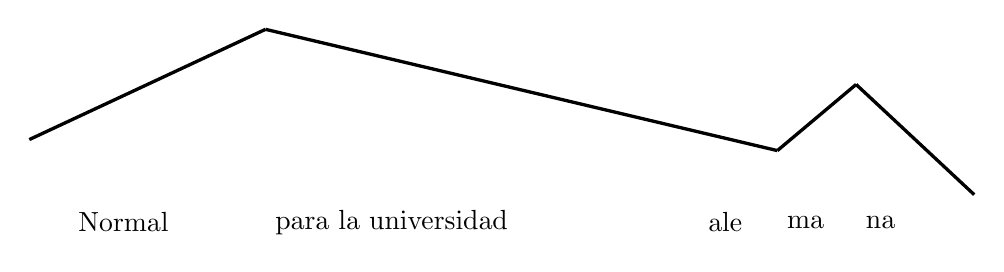
\begin{tikzpicture}[yscale = 0.7]
			\draw [very thick] (0,0.5) -- (3,2.5);
			\draw [very thick] (3,2.5) -- (9.5,0.3);
			\draw [very thick] (9.5,0.3) -- (10.5,1.5);
			\draw [very thick] (10.5,1.5) -- (12,-0.5);
			
			\node[anchor=west] at (0.5,-1) {Normal};
			\node[anchor=west] at (3,-1) {para la universidad};
			\node[anchor=west] at (8.5,-1) {ale};
			\node[anchor=west] at (9.5,-1) {ma};
			\node[anchor=west] at (10.5,-1) {na};
		\end{tikzpicture}
	\caption{Redundancy contour \textit{Normal para la universidad alemana.} `Normal for the German university.' \citep[20]{BeckmanETAL.2002}} 
	\label{fig:redundancycontourSPANISH}
\end{figure}


\begin{exe}
	\ex \label{ex:redundancycontourSPANISH} 
	Context \autoref{fig:redundancycontourSPANISH} \citep[19]{BeckmanETAL.2002}
	\begin{xlist}[A:]
	\exi{A:} A mí me parece normal que todo empiece a su hora. 
	\glt `I think it is normal for everything to start on time.'
	\exi{B:} Bueno, sí, \textit{normal, para la universidad alemana}. No para cualquier sitio, o también puede ser quizá normal para un alumno de alemán.
	\glt `Well, yeah, \textit{normal for the German university}. Not just for any place. Or maybe normal for a student of German.'
	\end{xlist}
\end{exe}

%\begin{figure}
%	\centering
%	
%	\includegraphics[width=.95\linewidth]{gfx/BeckmanETAL_2002_redundancy_contour.jpg}
%	\caption[Redundancy contour \textit{Normal para la universidad alemana.}]{Redundancy contour \textit{Normal para la universidad alemana.} `Normal for the German university.' \citep[20]{BeckmanETAL.2002}} 
%	\label{fig:redundancycontourSPANISH}
%\end{figure}


Their tentative description is ``an intonational idiom consisting of a pair of L+H* accents at the beginning and end of the target phrase, with no intervening accent.'' \citep[19]{BeckmanETAL.2002} In other words, they propose a correspondence between a holistic meaning (redundancy) and an intonational form /L+H* L+H* (L\%)/. Concerning this example, several questions remain unanswered. It seems as if its particular discourse meaning arises due to a mixture of agreement and disagreement between A and B. While B agrees with the normality of \textit{starting on time}, he disagrees with the realm of reference. He therefore starts by (partially) denying the previous assertion with \textit{bueno}, then proceeds to agree by using \textit{sí}, and then explains his partial disagreement by using this particular intonational contour. A decompositional approach would need to disentangle these different aspects.\largerpage

Concerning the state of the art, \autoref{tab:intonationalcategoriesGABRIEL} is more compositional than \autoref{tab:intonationalcategoriesPRIETO} since it attributes individual functions to tonal categories. Yet \autoref{tab:intonationalcategoriesGABRIEL} only covers the most prototypical cases of declaratives and interrogatives, allowing for four functional distinctions: focus, presupposition/topic, declarative, and interrogative.\footnote{Since /(L+H)*/ varies according to boundaries introduced either by phrase accents or boundary tones (or in free variation in the case of L*), it does not carry informational load of its own and renders contrastive /L+H*/ phonetically identical to a /(L+H)*/ followed by /L$-$/. Since \%H is facultative, the four meaningful categories are /L+H*/, /H$-$/, /L\%/, and /H\%/.} Less prototypical sentence types in Spanish have so far only received a holistic treatment. 

%\subsection{Compositional approaches to English intonation}
%\label{ch:2.3.2}
%
%To illustrate more complex compositional approaches, a detour to accounts of languages other than Spanish is necessary. English intonation has received a treatment that explicitly sets out to be compositional. The seminal paper by \citet{PierrehumbertHirschberg1990} precisely defines how such an approach needs to proceed, without necessarily succeeding in doing so. A recapitulation of their argument is still helpful, though, for showing the spirit that guides compositional approaches to intonation. They search for a ``comforting parallelism between the prosodic domain on which an intonational morpheme is realized, and the kind of meaning it has'' \citep[222]{Buring.2016}.
%
%\begin{displayquote}
%	Pitch accents, phrase accents, and boundary tones each operate on a 
%	(progressively higher) domain of interpretation. Not only is each of 
%	these types of tone interpreted over a distinct	domain, but each 
%	contributes a distinct type of information to the overall 
%	interpretation of a tune. \citep[286]{PierrehumbertHirschberg1990}
%\end{displayquote}
%
%\citet{PierrehumbertHirschberg1990} partially decompose pitch accents into 
%monotonal alignment and bitonal combinations of alignment and slope. H* 
%alignment signals to the hearer ``that the open expression is to 
%be instantiated by the accented items and the instantiated proposition 
%realized by the phrase is to be added to [the hearers] mutual belief 
%space.'' \citep[290]{PierrehumbertHirschberg1990} L* alignment, in turn, excludes an item from this kind of 
%``predication''. Bitonal pitch accents are attributed an additional meaning according to their slope. A rise evokes a salient 
%scale, whereas a fall evokes the possibility of an inference related to 
%the accented item.\footnote{\citet{PierrehumbertHirschberg1990} do not explain if rise and fall can combine to form a tritonal pitch accent that would denote [$+$predication,$+$inference,$+$scale].} The combinatorics of monotonal 
%meanings and bitonal slopes result in the six pitch accent meanings 
%repeated in \autoref{tab:accentmeaningPH} (adapted from 
%\cite[236]{Buring.2016}).

%\begin{table}
%	\begin{tabularx}{\textwidth}{llYlcc}
%		\lsptoprule
%		& & & & \multicolumn{2}{c}{\textsc{slope}}  \\
%		& & & & rise L$+$H & fall H$+$L \\
%		\multirow{2}{*}{\textsc{pitch accent}} & H* & $+$predication & H* 
%		& 
%		L$+$H* & H*$+$L	\\
%		& L* & -predication & L* & L*$+$H & H$+$L* \\ 
%		\lspbottomrule
%	\end{tabularx}
%	\caption[Pitch accent meanings in 
%	\citet{PierrehumbertHirschberg1990}]{Pitch accent meanings in 
%		\citet{PierrehumbertHirschberg1990}.}
%	\label{tab:accentmeaningPH}
%\end{table}


%\begin{table}
%	\begin{tabularx}{\textwidth}{llXXX}
%		\lsptoprule
%		 & & & \multicolumn{2}{c}{\textsc{Slope}}  \\
%		 & & & rise L$+$H & fall H$+$L \\
% 		\cmidrule{3-5}
%		 & &\textsc{Meaning} & scale & inference \\
%		\cmidrule{3-5}
%		\multirow{2}{*}{\textsc{Align}} & H* & $+$predication & 
%		$+$predication 
%		$+$scale & $+$predication $+$inference \\
%		 & L* & $-$predication & $-$predication $+$scale & 
%		$-$predication $+$inference \\ 
%		\lspbottomrule
%	\end{tabularx}
%	\caption[English pitch accent meanings]{English pitch accent meanings in \citet{PierrehumbertHirschberg1990}.}
%	\label{tab:accentmeaningPH}
%\end{table}
%
%Phrase accents and boundary tones indicate the presence/absence of an 
%interpretive boundary \citep[302--308]{PierrehumbertHirschberg1990}. H$-$ and H\%
%link an \ac{ip}/\ac{IP} to the following \ac{ip}/\ac{IP}, 
%whereas an L$-$ or L\% separates the two (or lacks a linking function). As already noted by \citet[321--322]{Hobbs.1990}, the characterization 
%of \ac{T-} and \ac{Tpercent} as cata- and anaphoric falls short of 
%recognizing the hierarchical structure of discourse according to layers of 
%\ac{QUD}.
%\footnote{See \citet{BuchholzUNDERREVIEW} for an approach to Peruvian Spanish and Quechua intonation using QUD.}

%All in all, many of the meanings referred to in \citet{PierrehumbertHirschberg1990} are vague and 
%lack the incorporation into a model of discourse meaning. But the main 
%insight remains untouched: compositionality of tonal structure reduces the amount of basic meanings 
%and creates complex meanings by combining tonal morphemes with each other 
%and with segmental meanings. \citet[246--247]{Steedman.2007} has translated the proposal by \citet{PierrehumbertHirschberg1990} to the following three dimensions: Common Ground presupposition (theme) vs. Common Ground update (rheme), $\pm$\textsc{a\-greed}, and speaker commitment vs. hearer attribution. Rising pitch accents presuppose the denotation of a constituent, while monotonal or falling accents propose an update of the \ac{CG}. High alignment (H*) denotes $+$\textsc{agreed}, while low alignment (L*) denotes $-$\textsc{a\-greed}.\footnote{\citet[26--27]{Steedman.2014} replaces $\pm$\textsc{a\-greed} with success and failure, which I take to be less transparent terms.} Finally, high boundary tones are hearer-attributed, while low boundary tones denote speaker commitment. While this perspective is not formalized dynamically in terms of context updates, I take it to be a major step towards an understanding of intonation in terms of discourse contexts that take into account the public commitments of interlocutors, their relations of (dis)\-a\-gree\-ment about propositions, and their current and future Common Ground. In \sectref{ch:3.3}, I will present a model that is partially based on these ideas.

\subsection{The Provocation-Response Nexus}

This is true not only for Spanish, but also for French. Building on the seminal paper by \citet{PierrehumbertHirschberg1990} and its adaptation by \citet{Steedman.2007}, there has been a lot of work on the meanings encoded by French intonation \citep{BeyssadeMarandin.2009,PortesBeyssade.2012,PortesReyle.2014,PortesBeyssadeMichelasMarandinChampagneLavau.2014,MichelasPortesChampagneLavau.2016}. Yet in the treatment of marked speech acts, such as the implication contour \citep{Delattre1966} as investigated by \citet{PortesBeyssadeMichelasMarandinChampagneLavau.2014}, we again find that the level of description is rather on the level of tunes than on individual tones. \citet{PortesBeyssadeMichelasMarandinChampagneLavau.2014} found that speakers chose different types of reactions depending on the final contours of the previous declarative \textit{Jules a engagé un ingénieur} (`Jules hired an engineer'). Declaratives ending in ``conclusive intonation'' L* L\% (\ref{ex:portesbeyssademichelasmarandinchampagnelavauLL}) led listeners to choose the reaction \textit{J'en prends note} (`I get it'). On the contrary, the ``implication contour'' H* L\% led to the reaction \textit{J'en sais rien} (`I've no idea about it') (\ref{ex:portesbeyssademichelasmarandinchampagnelavauHH}).\footnote{This response was also preferred in reaction to the ``question'' contour H* H\%.} Finally, the ``incredulous reply'' H+!H* H\% statements were met with \textit{Si, si, je t'assure} (`No, really, it's true') (\ref{ex:portesbeyssademichelasmarandinchampagnelavauDOWNSTHH}). Note that here, much as for Spanish nuclear configurations, we make reference to sequences of simple or complex pitch accents and boundary tones, not to correspondences between individual tones and meanings.\largerpage

\begin{exe}
\ex \label{ex:portesbeyssademichelasmarandinchampagnelavauLL} ``conclusive intonation'' (French) 
	\begin{xlist}[A:]
	\exi{A:} Jules a engagé un ingénieur. L* L\% 
	\glt `Jules hired an engineer.' 
	\exi{B:} J'en prends note. 
	\glt `I get it.' 
	\end{xlist}

\ex \label{ex:portesbeyssademichelasmarandinchampagnelavauHH} ``implication contour'' (French)
	\begin{xlist}[A:]
		\exi{A:} Jules a engagé un ingénieur. H* L\% 
		\glt `Jules hired an engineer.' 
		\exi{B:} J'en sais rien. 
		\glt `I've no idea about it.' 
	\end{xlist}

\ex \label{ex:portesbeyssademichelasmarandinchampagnelavauDOWNSTHH} ``incredulous reply'' (French)
	\begin{xlist}[A:]
		\exi{A:} Jules a engagé un ingénieur. H+!H* H\% 
		\glt `Jules hired an engineer.' 
		\exi{B:} Si, si, je t'assure. 
		\glt `No, really, it's true.' 
	\end{xlist}
\end{exe}

These findings show that variability in the prosodic form of a declarative can have a strong impact on the kind of response the interlocutor will choose. Note that we are not dealing with question-answer pairs, but pairs of statements that nevertheless differ in conversational initiative.\footnote{The model is introduced in \sectref{ch:3.3}. Conversational initiative is defined there as the act of commitment to the content of a speech act which raises an issue that requires a reaction (or tacit agreement) to be settled.} I will refer to sentences such as those uttered by A in these examples as \textit{provocations}.\footnote{These are also called ``first pair parts'' in the literature on adjacency pairs \citep{SacksSchegloffJefferson.1974,SchegloffSacks.1973}.} Replies such as those uttered by B will be called \textit{responses} \citep{FarkasBruce.2010}.

A declarative can serve as a provocation, proffering a proposition as true and adding information about the way it relates to the discourse context as composed of the commitments of the speaker, the hearer(s), and the Common Ground by way of its prosodic makeup. The response can then react to the proffered content. If the reaction targets the proffered content directly, non-at-issue markers such as intonation can serve to evaluate the reaction. Finally, in the case of a prosodically marked provocation, the response can also switch tack and react to the additional, prosodic information. To capture this complex relation, (\ref{ex:provocationresponsenexus}) defines the intonational \textit{Provocation-Response Nexus}. It is stated as a broad concept here, but will be illustrated and discussed more precisely in \sectref{ch:3.3.3}.

\begin{exe}
	\ex \label{ex:provocationresponsenexus} \textit{Intonational Provocation-Response Nexus} \\
	Marked intonation on a response is meaningful relative to its provocation.
\end{exe}

%unbefriedigend!
%Non-at-issue content in provocations, expressible via intonation amongst other means, leads to marking in the response that also corresponds to non-at-issue content

\subsection{Spanish intonational phonemes}
\label{ch:2.3.3}

As stated above, research on Spanish intonation has paid a lot of attention to the different meanings encoded by nuclear contours, yet without an explicit theory of intonational meaning.\footnote{Even though \citet{EscandellVidal.1998} made some early contributions to the differentiation between neutral, hearer attributed, and speaker attributed polar questions, a finding corroborated by \citet{HenriksenArmstrongGarciaAmaya.2016}.} The occurrence of specific pitch accents, phrase accents, and boundary tones in different positions and sentence types was meti\-cu\-lously do\-cu\-men\-ted, leading to a proliferation of tonal categories with varying degrees of distributional flexibility. \autoref{tab:pitchaccentsSPANISH} gives an overview based on \citet{Aguilar.2009} of different pitch accents and their distribution pattern.\footnote{These are often called intonational morphemes \citep{Gussenhoven.2016}, but rather have the status of phonemes in holistic approaches such as the one presented here \citep[219--223]{Buring.2016}. I thank an anonymous reviewer for pointing this out.} \autoref{tab:phraseacacentsSPANISH} does the same for phrase accents and \autoref{tab:boundarytonesSPANISH} for boundary tones.

\begin{table}
	\begin{tabular}{l@{~~}lll}
		\lsptoprule
		\multicolumn{2}{l}{Pitch accent}   &  Sentence type & Nuclearity \\
		\midrule
		a. & H* & \textit{wh}-questions & nuclear\\
		   & & polite yes-no questions & nuclear\\
		b. & L* & broad focus statements & nuclear\\
		c. & H+L* & confirmatory yes-no questions & nuclear\\
		   & & imperative yes-no questions & nuclear \\
		d. & L+¡H* & counter-expectational questions & nuclear\\
		e. & L+H* & broad/narrow focus statements & nuclear \\
		   & & vocatives & nuclear\\
		   & & insistent requests & nuclear\\
		   & & statements of the obvious & nuclear\\	
		f. & L*+H & yes-no questions & prenuclear \\
		   & & requests & prenuclear\\
		g. & L+<H* & broad focus statements & prenuclear \\
		\lspbottomrule 
	\end{tabular}
	\caption{Previous findings on Spanish pitch accents 
	by sentence type \citep{Aguilar.2009}}
	\label{tab:pitchaccentsSPANISH}
\end{table}

\begin{table}
	\begin{tabularx}{\textwidth}{l@{~~}lX}
		\lsptoprule
		\multicolumn{2}{l}{Phrase accent}   &  Occurrence \\
		\midrule
		a. & L$-$ & after left- and before right-dislocated elements\\
		b. & M$-$/!H$-$ & in pedagogic enumerations; after clefted foci in questions \\
		c. & H$-$ & at the end of non-final constituents, inconclusive statements, etc. \\
		d. & HH$-$ & at the end of the first part of alternative questions \\
		e. & LH$-$ & in anti-expectational/incredulity questions and statements of the obvious \\
		f. & HL$-$ & in exhortative requests and statements of the obvious \\
		g. & LHL$-$ & in exhortative requests \\
		\lspbottomrule 
	\end{tabularx}
	\caption{Previous findings on Spanish phrase accents by sentence type \citep{Aguilar.2009}\label{tab:phraseacacentsSPANISH}}
\end{table}

\begin{table}
	\begin{tabularx}{\textwidth}{l@{~~}lX}
		\lsptoprule
		\multicolumn{2}{l}{Boundary tone}  &  Occurrence \\
		\midrule
		a. & L\% & broad and narrow focus statements, imperatives, 
		anti-expectational and imperative yes-no questions, \textit{wh}-questions, 
		etc. \\	
		b. & M\% & pedagogic enumerations, hesitation statements, polite 
		yes-no questions, stylized vocatives (+lengthening) \\		
		c. & HH\% & yes-no questions \\
		d. & LH\% & anti-expectational and invitation questions \\
		e. & LM\%/L!H\% & statements of the obvious \\
		f. & HL\% & contrastive focus with obviousness nuance \citep[279]{EstebasVilaplanaPrieto.2008}, exhortative requests, emphatic exclamatives and insistent vocatives \\
		g. & LHL\% & exhortative requests \\
		\lspbottomrule 
	\end{tabularx}
	\caption{Previous findings on Spanish boundary tones by sentence type \citep{Aguilar.2009}\label{tab:boundarytonesSPANISH}}
\end{table}

Taken together, Tables~\ref{tab:intonationalcategoriesPRIETO} and~\ref{tab:pitchaccentsSPANISH} show that the focus on sentence types leads to a phonological perspective in which nuclear configurations become the sorting category on which both the tonal inventory and the functional descriptions depend. Yet nuclearity is a problematic category. Dating back to the Nuclear Stress Rule by \citet[17]{ChomskyHalle.1968}, which explicitly claims automatic rightmost primary stress for syntactic phrases in English, a strict view on prominence assignment has persisted in parts of the literature on Spanish (e.g. \cite{Zubizarreta.2016}). As mentioned in \sectref{ch:2.2.2}, Spanish cannot simply be classified as a ``word order language'' as opposed to ``intonation languages'' such as German. Yet nuclearity as used in the literature on Spanish intonation is still mostly interpreted as \ac{IP} finality in terms of the end of a turn, often in the form of a sentence. Moreover, the difference between \ac{T-} and \ac{Tpercent} is blurred in cases of bi- or tritonal boundaries. Are the bitonal HL\% and HL$-$, found in exhortative requests, statements of the obvious, and contrastive focus with obvious nuances, actually two different phonemes? Are they different from LHL$-$ and LHL\%? 
%\autoref{fig:exhortative} and \autoref{fig:exhortative_long} give the impression tritonal LHL\% boundary tones are different associations of the same tonal sequence as combinations of monotonal L* pitch accents with bitonal HL\% boundary tones. 

A similar question arises in the comparison of LH$-$ and LH\% in anti-ex\-pec\-ta\-tio\-nal questions and obviousness statements. Moreover, this similarity raises the question about what it means for a question to be anti-expectational and for a statement to be obvious. We need a semantic criterion that distinguishes LM\%/L!H\% from LH\% to know if the phonological distinction holds. Continuing this line of thought, an understanding of HL\% requires a definition of emphatic exclamatives and insistent vocatives, particularly if we want to maintain the idea that HL$-$ can be found in obviousness statements. In the attempt to establish the intonational phonemes of Spanish, two problems seem to mutually reinforce each other. On the one hand, variability of tonal association leads to a proliferation of tonal categories. On the other hand, subtle meanings beyond the declarative-interrogative and focus-background dichotomies seem important, yet are poorly understood. This becomes particularly clear when looking at larger data sets.

%Finally, given that syntax does not distinguish between \autoref{fig:pregunta_informativa} and \autoref{fig:pregunta_abs_conf}, we could ask what it is that renders them interrogatives instead of declaratives. 

%\begin{figure}
%	\centering
%	\includegraphics[width=.95\linewidth]{gfx/figure_exhortative_request.jpg}
%	\caption[Exhortative request \textit{¡Venga, va!}]{Exhortative request 
%		\textit{¡Venga, va!} `Come on, please!' 
%		\citep{Aguilar.2009}. \href{http://prosodia.upf.edu/sp_tobi/sound_files/mp3/11.mp3}{\faVolumeUp} \href{http://prosodia.upf.edu/sp_tobi/en/exercises/solutions/tonal_representation/NC_recognition.html}{\faExternalLink*}} \label{fig:exhortative}
%	\bigskip
%	\includegraphics[width=.95\linewidth]{gfx/figure_exhortative_request_long.jpg}
%	\caption[Exhortative request \textit{¡Va, vente, hombre!}]{Exhortative 
%		request \textit{¡Va, vente, hombre!} `Come on, come over, dude!' 
%		\citep{Aguilar.2009}. \href{http://prosodia.upf.edu/sp_tobi/sound_files/mp3/va-vente-hombre.mp3}{\faVolumeUp} \href{http://prosodia.upf.edu/sp_tobi/en/exercises/solutions/tonal_representation/NC_recognition.html}{\faExternalLink*}}\label{fig:exhortative_long}
%\end{figure}
%
%\begin{figure}
%	\centering
%	\includegraphics[width=.95\linewidth]{gfx/figure_pregunta_informativa.png}
%	\caption[Pregunta absoluta informativa \textit{¿Tiene mermelada?}]{Pregunta 
%		absoluta informativa \textit{¿Tiene mermelada?} `You have marmalade?' 
%		\citep{Prieto2009-2013}. \href{http://prosodia.upf.edu/atlasentonacion/enquestes/espanol/madrid/frases/mp3/11.mp3}{\faVolumeUp} \href{http://prosodia.upf.edu/atlasentonacion/enquestes/espanol/madrid/index.html}{\faExternalLink*}}\label{fig:pregunta_informativa}
%	\bigskip
%	\includegraphics[width=.95\linewidth]{gfx/figure_pregunta_absoluta_confirmacion.png}
%	\caption[Pregunta absoluta de confirmación \textit{¿Tienes frío?}]{Pregunta 
%		absoluta de confirmación \textit{¿Tienes frío?} `You're could?' 
%		\citep{Prieto2009-2013}. \href{http://prosodia.upf.edu/atlasentonacion/enquestes/espanol/madrid/frases/mp3/15.mp3}{\faVolumeUp} \href{http://prosodia.upf.edu/atlasentonacion/enquestes/espanol/madrid/index.html}{\faExternalLink*}}\label{fig:pregunta_abs_conf}
%\end{figure}

\subsection{Variable intonation on Spanish insubordinates}\label{ch:2.3.4}\largerpage

In an exceptionally large-scale study of Spanish intonation, \citet{ElviraGarcia.2016} investigates the prosody of insubordinate clauses in Spanish. In total, nineteen types of insubordinates are investigated, based on the combination of six conjunctions/particles (some commencing only with \textit{si} `if/but/well' or \textit{que} `that', others with combinations such as \textit{como si} `as if', \textit{ni que} `not even that', etc.). For those insubordinations that allow it, both indicative and subjunctive verbal mood are tested \citep[58]{ElviraGarcia.2016}. See (\ref{ex:perosiVind}) for an example with indicative mood, and (\ref{ex:comosiVsub}) together with \autoref{fig:comosiVsubFIGURE} for an example with subjunctive verbal mood \citep[324--325]{ElviraGarcia.2016}.\footnote{See \sectref{ch:6.1.2} for a discussion and application of Eti\_ToBI, the tool developed by \citet{ElviraGarcia.2016,ElviraGarciaRoseanoFernandezPlanas.2016} to generate these tonal analyses. Two additional phonetic transcription tiers are omitted here for convenience.}


\begin{exe}
	\ex  \label{ex:perosiVind}  CONTEXTO: Eres la canguro de dos niñas, una de las niñas está comiendo	chuches a las 5 de la tarde y, entonces, viene la otra hermana (que soy yo) a	chivarse y te digo: \\
	ENTREVISTADORA: Marina está comiendo cuches \\
	RESPUESTA: ¡Pero si va a merendar!
	
	\glt `CONTEXT: You're the nanny of two girls, one of the girls is eating sweets at 5 pm and then the other sister (which is me) to snitch and I tell you:' \\
	`INTERVIEWER: Marina is eating sweets' \\
	`RESPONSE: ¡But SI she is going to have lunch!'

\ex  \label{ex:comosiVsub}  CONTEXTO: Imagina que soy tu canguro y la de tu hermana. Tú quieres pasar
	una temporada sin merendar para adelgazar y yo no te dejo y te digo... \\
	ENTREVISTADORA: Mira, tu hermana está delgada y sin \\ 
	dejar de tomar ninguna comida \\
	CONTEXTO: Pero tú sabes que ella no merienda \\
	(lo tira a la basura), y me respondes:... \\
	RESPUESTA: ¡Como si merendara médula! 
	
	\glt `CONTEXT: Imagine that I'm the nanny of you and of your sister. You want to skip lunch for a while to lose weight, but I don't let you and tell you ``Look your sister is thin without skipping meals'', but you know that she doesn't have lunch (she throws it away), and you answer me...'\\
	`RESPONSE: As if she'd be having meat-soup for lunch!'
\end{exe}


\begin{figure}
		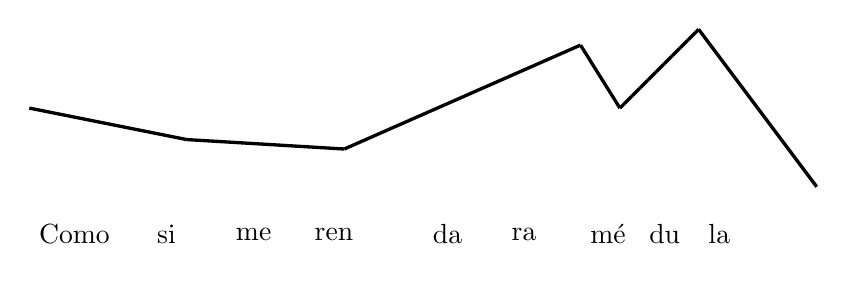
\begin{tikzpicture}[yscale = 0.8]
			\draw [very thick] (0,1.5) -- (2,1);
			\draw [very thick] (2,1) -- (4,0.85);
			\draw [very thick] (4,0.85) -- (7,2.5);
			\draw [very thick] (7,2.5) -- (7.5,1.5);
			\draw [very thick] (7.5,1.5) -- (8.5,2.75);
			\draw [very thick] (8.5,2.75) -- (10,0.25);
						
			\node[anchor=west] at (0,-0.5) {Como};
			\node[anchor=west] at (1.5,-0.5) {si};
			\node[anchor=west] at (2.5,-0.5) {me};
			\node[anchor=west] at (3.5,-0.5) {ren};
			\node[anchor=west] at (5,-0.5) {da};
			\node[anchor=west] at (6,-0.5) {ra};
			\node[anchor=west] at (7,-0.5) {mé};
			\node[anchor=west] at (7.75,-0.5) {du};
			\node[anchor=west] at (8.5,-0.5) {la};
		\end{tikzpicture}
	\caption{\textit{¡Como si merendara médula!} `As if she'd be having meat-soup for lunch!' \citep[120]{ElviraGarcia.2016}.}\label{fig:comosiVsubFIGURE}
\end{figure}

% \begin{figure}
% 	\centering
% 	\includegraphics[width=.95\linewidth]{gfx/figure_como_si_120_ELVIRA_GARCIA.jpg}
% 	\caption[\textit{¡Como si merendara médula!}]{\textit{¡Como si merendara médula!} `As if she'd be having meat-soup for lunch!' 
% 		\citep[120]{ElviraGarcia.2016}.}\label{fig:comosiVsubFIGURE}
% \end{figure}


In her examples, the subordinating conjunction/insubordinating particle is integrated into the same intonation unit as the main declarative clause. Even though I translate \textit{si} with `if', this is actually not correct because it functions as an adversative marker. Yet neither can it be translated as `but', because it does not express \textit{restrictive adversativity} (or PA adversativity, \citealt{AnscombreDucrot.1977}). Moreover, for sentences with indicative verbal mood, \citet[22]{Schwenter.2016} found that it cannot simply be translated with `but rather' either (also called SN or \textit{corrective adversativity}), since it adds non-truth conditional meaning which marks ``the proposition that it accompanies as one that is obviously true to the speaker.''\footnote{It is therefore possible, and even common, to have a sequence of two adversative conjunctions and particles such as \textit{pero si}, which combine the adversative meanings of both. See \sectref{ch:5.2.1} for the very common sequence \textit{hombre si}.}\largerpage

\citet{ElviraGarcia.2016} deserves to be discussed at length here for at least three reasons. Firstly, the study is an impressive example for the way in which intonation research can go beyond the discussion of individual examples by a series of interactive discourse completion task experiments and a partial automation of ToBI transcription. Even more importantly for the discussion of distinctive functions of intonation, the study is also a prime example of how a relatively reduced interest in meanings such as obviousness can make it more difficult to interpret a wealth of important empirical results.

In an attempt to control for tonal crowding effects, \citet[54--56]{ElviraGarcia.2016} varies the metrical structure (and syllabic structure in case of ultimate stress) of the final prosodic word with examples such as (\ref{ex:perosiVX}). (\ref{ex:perosiVX}) is supported by a stimulus that shows a girl (Marina) eating a carrot. This is an important detail, because such a stimulus gives the participants a reason to reject the provocation independently of any general (shared) assumptions about Marina's diet.

\begin{exe}
	\ex  \label{ex:perosiVX}  CONTEXTO: Sabes que Marina merienda todos los días verdura.\\
	ENTREVISTADORA: Marina merienda chocolate.\\
	RESPUESTA:
	\begin{xlist}
		\ex ¡Pero si merienda \textbf{mé}dula! (antepenultimate) 
		\ex ¡Pero si merienda ver\textbf{du}ra! (penultimate) 
		\ex ¡Pero si merienda guara\textbf{ná}! (ultimate, $-$coda)
		\ex ¡Pero si merienda bibe\textbf{rón}! (ultimate, $+$coda)
	\end{xlist} 
	\glt `CONTEXT: You know that Marina is having vegetables for lunch every day.' \\
	`INTERVIEWER: Marina is having chocolate for lunch.'\\
	`RESPONSE:' 
	\begin{xlist}
		\ex `¡But SI she is having meat soup for lunch!' 
		\ex `¡But SI she is having vegetables for lunch!' 
		\ex `¡But SI she is having guaraná for lunch!' 
		\ex `¡But SI she is having a baby bottle for lunch!' 
	\end{xlist}
\end{exe}

For Madrid Spanish sentences of the form <si+V\textsubscript{IND}+O>, \citet[138--143]{ElviraGarcia.2016} finds only L* HL\% examples in sentences with antepenultimate stress on the final word. Sentences with penultimate stress on the final word have the same preference but also allow for L+H* L\% realizations. Finally, ultimate stress leads to truncation of the final low tone L+H*(L\%), which surfaces as L* H\%. 

While these results seem conclusive, the picture becomes much less clear when taking into account the whole set of insubordinates (e.g. introduced by \textit{como} `as',  \textit{ni que} `not that', \textit{que} `that', etc.). \autoref{tab:resultadosELVIRAGARCIAmadrid} shows the overall results for Madrid Spanish insubordinates. We see here that the tendency for the penultimate condition to prefer L* HL\% found for \textit{pero si} insubordinates has been reversed. If taken as a whole, the intonational form of insubordinates seems unstable in the penultimate condition. Given that the vast majority of words in Spanish have penultimate stress, this instability concerns a crucial point in the system. \citet[253–263]{ElviraGarcia.2016} discusses four possible explanations (\ref{ex:explanationsELVIRAGARCIA}).

\begin{table}
	\begin{tabular}{llrrrrr}
		\lsptoprule
		 & & \multicolumn{4}{c}{\textsc{final word stress}} & \\\cmidrule(lr){3-6}
		 & & ult. ($+$coda) & ult. & penult. & ante\-penult. & Total \\\midrule
		\multirow{3}{*}{\textsc{NI}} & L* HL\% & 4 & 11 & 23 & 125 & 163 \\
											   & L+H* HL\% & 0 & 0 & 0 & 5 & 5 \\
											   & L+H* L\% & 25 & 11 & 51 & 44 & 131 \\
											   & Total & 29 & 22 & 74 & 174 & 299 \\	 
		\lspbottomrule
	\end{tabular}
	\caption{\citet[254]{ElviraGarcia.2016} results for low-rise-fall in Madrid Spanish depending on accent type\label{tab:resultadosELVIRAGARCIAmadrid}}
\end{table}

\begin{exe}
	\ex \label{ex:explanationsELVIRAGARCIA}
	\begin{xlist}
		\ex retraction of an underlying L* HL\% to L+H* L\% in penult. and ult. condition
		\ex expansion of an underlying L+H* L\% to L* HL\% in antepenult. condition
		\ex variation according to the number of prosodic words in the phrase 
		\ex variation according to slightly different pragmatic functions
	\end{xlist}
\end{exe}

(\ref{ex:explanationsELVIRAGARCIA}a,b) both cannot explain the variability in the penultimate condition. (\ref{ex:explanationsELVIRAGARCIA}c) explains some tendencies for three-word utterances to prefer L+H* L\%, but is far from covering the variability in the data. Finally, (\ref{ex:explanationsELVIRAGARCIA}d) is discarded because the data does not show a ``complementary distribution'' \citep[253]{ElviraGarcia.2016}. 

I would argue that (\ref{ex:explanationsELVIRAGARCIA}d) deserves to be tested again, given that the data in \citet{ElviraGarcia.2016} has not been controlled at the semantic/pragmatic level and can reveal a complementary distribution only with regard to the categories tested. While it is without doubt a groundbreaking study in many regards, it still suffers from the lack of a theory of notions such as \textit{contradiction} and \textit{obviousness}. I take this to be one reason why the state of the art has always been inconclusive about contrastive focus and contradiction statements. While \autoref{tab:intonationalcategoriesPRIETO} takes L* HL\% to be the norm for contrastive focus and contradiction, \autoref{tab:intonationalcategoriesGABRIEL} sees L+H* L\% as the obligatory tonal--metrical association for contrastive focus. In their discussion of narrow-focus and epistemically biased statements, \citet[369]{HualdePrieto2015} state that ``although the overall shape of the contour is essentially the same (rise-fall), there is an important different alignment of the H with respect to the tonic, resulting in perceptually quite different contours. [\ldots] Where both nuclear contours are found, L* HL\% carries a greater emphatic, contradictory force.''

This becomes even more apparent when taking into account the L+H*L!H\% contour. \citet[258--260]{ElviraGarcia.2016} finds that in utterances with only one prosodic word (that is with one lexically stressable syllable), approximately one third of the realizations receives such a contour. Yet it also occurs in multi-word utterances, as in \autoref{fig:paraquemeriendeLHLHfigure}, contextualized in (\ref{ex:paraquemeriendeLHLH}) \citep[325--326]{ElviraGarcia.2016}.

\begin{exe}
	\ex  \label{ex:paraquemeriendeLHLH}  CONTEXTO: Tú sabes que siempre que llevo a Lorena a la carnicería se compra médula para merendar y a ti no te gusta ir a la carnicería pero piensas que si es por la médula de Marina [sic!] te tendrás que sacrificar.\\
	ENTREVISTADORA: Yo te digo que lleves a Marina a la carnicería y tú me respondes:\\
	RESPUESTA: ¡Sí, hombre! Para que meriende.
	\glt `CONTEXT: You know that I always take Lorena to the butcher's [for her to] buy herself some meat-soup for lunch and you don't like going there but think that when it comes to Marina's meat-soup you need to make that sacrifice.'\\
	`INTERVIEWER: I tell you to take Marina to the butcher's and you answer me:'\\
	`RESPONSE:	¡Sure, man! For her to have lunch.'
\end{exe}


\begin{figure}
		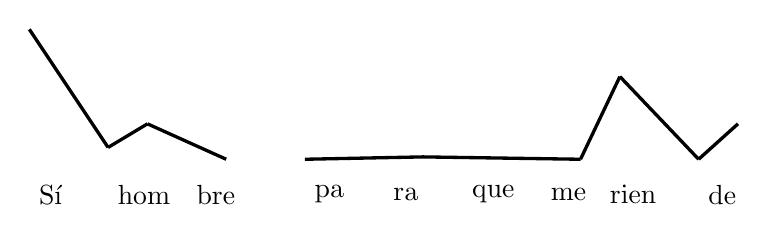
\begin{tikzpicture}[yscale = 0.6]
			\draw [very thick] (0.5,3) -- (1.5,0.5);
			\draw [very thick] (1.5,0.5) -- (2,1);
			\draw [very thick] (2,1) -- (3,0.25);
			\draw [very thick] (4,0.25) -- (5.5,0.3);
			\draw [very thick] (5.5,0.3) -- (7.5,0.25);
			\draw [very thick] (7.5,0.25) -- (8,2);
			\draw [very thick] (8,2) -- (9,0.25);
			\draw [very thick] (9,0.25) -- (9.5,1);
						
			\node[anchor=west] at (0.5,-0.5) {Sí};
			\node[anchor=west] at (1.5,-0.5) {hom};
			\node[anchor=west] at (2.5,-0.5) {bre};
			\node[anchor=west] at (4,-0.5) {pa};
			\node[anchor=west] at (5,-0.5) {ra};
			\node[anchor=west] at (6,-0.5) {que};
			\node[anchor=west] at (7,-0.5) {me};
			\node[anchor=west] at (7.75,-0.5) {rien};
			\node[anchor=west] at (9,-0.5) {de};
		\end{tikzpicture}
	\caption{\textit{¡Sí, hombre! Para que meriende.} `Sure, man! For her to have lunch.' \citep[129]{ElviraGarcia.2016}.}\label{fig:paraquemeriendeLHLHfigure}
\end{figure}

% \begin{figure}
% 	\centering
% 	\includegraphics[width=.95\linewidth]{gfx/figure_si_hombre_para_que_ELVIRA_GARCIA.jpg}
% 	\caption[\textit{¡Sí, hombre! Para que meriende.}]{\textit{¡Sí, hombre! Para que meriende.} `Sure, man! For her to have lunch.' \citep[129]{ElviraGarcia.2016}.}\label{fig:paraquemeriendeLHLHfigure}
% \end{figure}

While \citet[258--260]{ElviraGarcia.2016} discusses this prosodic configuration primarily as a phenomenon related to one-word utterances, such longer examples indicate that phrase length does not determine its occurrence. I therefore argue that a key factor is the presence of a context such as (\ref{ex:paraquemeriendeLHLH}) or (\ref{ex:perosiVind}) in which the reaction to the provocation does not challenge the at-issue content, but indicates that the provocation put well-established shared conventions up for discussion (e.g. \textit{No sweets before lunch}, \textit{Marina's soup is a priority}, etc.). This is quite different from contexts in which visual evidence (e.g. the picture of Marina eating a carrot) allows participants to correct the provocation.

While different contexts induce different meanings such as (dis)\-a\-gree\-ment and expectations, the same holds for the different forms of insubordination in Spanish. \citet[62, 323--325]{ElviraGarcia.2016} intuitively integrates this fact by adding particles to some of the target sentences which support the respective meanings, as in (\ref{ex:corpusELVIRAGARCIA}).

\begin{exe}
	\label{ex:corpusELVIRAGARCIA}
	\ex ¡\textit{Sí, hombre}! ¡Para que meriende verdura!
	\glt `\textit{Sure, man}! For her to have meat-soup for lunch'
	
	\ex \textit{Pues}, ¡que merienden médula!
	\glt `\textit{Well} let them have meat-soup for lunch'
	
	\ex ¡\textit{Anda}! ¡Si merienda!
	\glt `\textit{Wow}! SI she's having lunch!'
\end{exe}

Relatively consistent findings for individual insubordinates such as <pero si + V\textsubscript{IND} + O>, as compared to the rather inconsistent global results in \autoref{tab:resultadosELVIRAGARCIAmadrid}, indicate that the choice of a particular context for elicitation, combined with the meaning of the preceding particles and the meaning of the insubordinating form, triggers specific pragmatic interpretations which determine the intonational form of the utterances. And as long the pragmatics involved in this process are not fully understood, investigations of their form of expression run the risk of lumping together slightly different meanings and then taking differences in form as a sign of phonologically determined (or free) variation.

Before we turn to a model that attempts to provide such an understanding in \chapref{ch:3}, I end \chapref{ch:2} with a discussion of a more recent proposal for a new way of doing intonational phonology based primarily on Spanish obviousness contours.

\subsection{A melodic construction for obviousness?}
\label{ch:2.3.5}

Taking example (\ref{ex:claroesquedeesoTORREIRAGRICE}) from the Nijmegen Corpus of Casual Spanish \citep{TorreiraErnestus.2012} as a point of departure, \citet{TorreiraGrice.2018} argue that speakers of Peninsular Spanish choose different metrical associations of the /LHL/ tonal sequence depending on the length of the target phrase and the proximity between lexical stresses and prosodic boundaries. Example (\ref{ex:claroesquedeesoTORREIRAGRICE}) is taken from the discussion between two speakers from Madrid about the treatment of boys and girls in school. Speaker 2RM marks that his statement should ``be beyond any doubt by using the interjection \textit{claro} [as well as] by using the low-rise-fall in at least three out of the four phrases in this turn (as opposed, for instance, to a rising-falling declarative tune which would not have conveyed the same sense of obviousness [\ldots])'' \citep[16]{TorreiraGrice.2018}.\pagebreak

\begin{exe}
\ex\label{ex:claroesquedeesoTORREIRAGRICE} NCCSp\_02\_3494
\begin{xlist}
	\ex
	2RM: Pero en el colegio les tienes que tratar igual, o sea \ldots\\
	\hspace*{2em} `But in school you should treat them in the same way, I mean \ldots'
	\ex
	2CM: En nivel educa[tivo, que aprendan lo mismo].\\
	\hspace*{2em} `At the educational level, they should learn the same.'
	\ex
	2RM: \hspace{7em}[En educación, la educación,]\\
	\hspace*{9em} `In terms of education, education,'
	\ex
	2CM: Que aprendan lo mismo.\\
	\hspace*{2em} `They should learn the same.'
	\ex
	2RM: ¡\textbf{CLA}ro! \hspace{2em} ¡\textbf{Es} que \textbf{es} \textbf{e}so! \\
	\hspace*{3em} L* H(L\%) \\
	\hspace*{2em} `Of course! \hspace{1.5em} That's it!'\\
	\hspace*{2em} ¡\textbf{Es} que de \textbf{e}so se e\textbf{stá} ha\textbf{BLAN}do! ¡De educa\textbf{CIÓN}! \\
	\hspace*{2em} L* \hspace*{9.6em} H* L\% \hspace{4em} L* H(L)\% \\
	\hspace*{2em} `That's what's being discussed! \hspace{2.5em} Education!'
\end{xlist}
\end{exe}

As indicated in (\ref{ex:claroesquedeesoTORREIRAGRICE}e), only the multi-word phrase with penultimate stress rea\-ches a final low tone. And while the authors do not mention the similar findings by \citet{ElviraGarcia.2016}, the three low-rise-fall sequences in (\ref{ex:claroesquedeesoTORREIRAGRICE}e) still ``strike the attentive native listener [the researcher] as functionally equivalent at the intonational level'' \citep[16]{TorreiraGrice.2018}.

\citet{TorreiraGrice.2018} go on to show that L1 speakers of Italian with high L2 proficiency in Spanish differ from native speakers of Spanish and that they do not succeed in imitating the difference between a reduced fall in case of an HL\% association in single-word utterances (\ref{ex:claroTORREIRAGRICE}) and a fully realized fall in case of an H* L\% association in two-word utterances (\ref{ex:hermanodemanolo}) and three-word utterances (\ref{ex:amigahermanodemanolo}) with non-ultimate lexical stress in nuclear accent position.

\begin{exe}
	\ex \label{ex:claroTORREIRAGRICE}
	\textbf{CLA}ro, Ma\textbf{NO}lo. \\
	\hspace*{1em}L* H(L)\% \hspace*{0.2em} L* H(L)\% \hfill Spanish and Italian speakers
	\glt `Of course, Manolo.'

\ex \label{ex:hermanodemanolo}
	\textbf{CLA}ro, el her\textbf{ma}no de Ma\textbf{NO}lo. \\
	\hspace*{1em}L* H(L)\%\hspace*{5.2em} L+H* L\% \hfill Spanish speakers \\
        \hspace*{1em}L* H(L)\%\hspace*{6.5em} L* H(L)\% \hfill Italian speakers 
	\glt `Of course, Manolo's brother.'  
\pagebreak
\ex \label{ex:amigahermanodemanolo}
	\textbf{CLA}ro, la a\textbf{mi}ga del her\textbf{ma}no de Ma\textbf{NO}lo. \\
	\hspace*{1em}L* H(L)\%\hspace*{9.4em} L+H* L\% \hfill Spanish speakers \\
        \hspace*{1em}L* H(L)\%\hspace*{10.5em} L* H(L)\% \hfill Italian speakers 
	\glt `Of course, Manolo's brother's (girl)friend.' 
\end{exe}

Theoretically, they account for these findings by proposing a strict separation of the tonal and metrical tiers in \ac{AM}-phonology, together with \textit{melody-specific} principles of tonal--metrical association. To allow for these principles to be specific to a certain melody, they propose to model them as constructions in the sense of \citet{KayFillmore.1999,Croft.2001,Jackendoff.2002,Goldberg.2006}. As such, they do not contain fixed metrical information, but rather consist of a sequence of tones with principles of tonal--metrical association, together with a meaning specification that makes simultaneous reference to discourse context (discourse meaning) and syntax \citep[28--29]{TorreiraGrice.2018}. For the low-rise-fall /LHL/, they propose an obviousness meaning and three association rules (\ref{ex:lowrisefallRULES}).\footnote{I take it to be no coincidence that \citet{TorreiraGrice.2018} develop their proposal based on a tune which they take to communicate ``obviousness''. They draw their inspiration from the discussion about the difference in English between \textit{contradiction contours} and \textit{contrastive accents} dating back to \citet{LibermanSag.1974} and \citet{Grice.1995}. It seems as if the distinction between \textit{contrast} and \textit{contradiction} should receive as much attention in English intonational phonology as it should for Spanish.}

\begin{exe}
\ex\label{ex:lowrisefallRULES} low-rise-fall (obviousness) /L$_1$H$_1$L$_2$/ 
\begin{xlist}
	\ex L$_1$:
	\begin{xlist}
		\ex associate with the first stressed syllable of the ip 
		\ex spread rightwards up to the last stressed syllable of the ip 
	\end{xlist}
	\ex H$_1$: 
	\begin{xlist}
		\ex if N$_\omega \geq 2$ associate with the last stressed syllable of ip 
		\ex if N$_\omega = 1$ associate with the right edge of the ip 
	\end{xlist}
	\ex  L$_2$: associate with the right edge of the ip 
\end{xlist}
\end{exe}

Such flexibility in tonal association seems desirable given the apparent overlap in the inventories of Spanish intonational phonemes in Tables~\ref{tab:pitchaccentsSPANISH}--\ref{tab:boundarytonesSPANISH}. Unfortunately, this algorithm based on phrase-length measured in $\omega$ seems to be contradicted by the findings in \citet[142--143, 253--260]{ElviraGarcia.2016} as well as \chapref{ch:5}, which clearly show that H$_1$ can also associate with the right edge of the ip if N$_\omega \geq 2$.\footnote{\citet[142]{ElviraGarcia.2016} finds L*~HL\% to be the most frequent contour on insubordinates of the form \textit{¡Si merienda!} `But she is having lunch!'. \chapref{ch:6} finds non-truncated L*~HL\% on multi-word \acp{IP}.} So while the phrase-length based proposal would need to be refined if we take the findings by \citet{ElviraGarcia.2016} and in \chapref{ch:5} to concern the same meaning as in \citet{TorreiraGrice.2018},\footnote{Perhaps Spanish native speakers see \textit{Manolo} as an answer that is more likely to be obvious than \textit{Manolo's brother's (girl)friend} and adjust their prosody accordingly, whereas non-native speakers are less aware of the intonational meaning.} the idea of an association between specific meanings and tones (tonal sequences) which receive their association based on additional factors such as metrical structure and phrase length is still a viable possibility that could reduce the size of the inventory of intonational phonemes. 

My main point is that melodic constructions, just as nuclear configurations, can only be defined relative to shared meaning. As long as we lack a semantic model to predict intonational marking (be it in the form of tonal sequences with rules of tonal--metrical association or in the form of pitch accents, phrase accents, and boundary tones), there is no way of deciding on the required inventory of phonological categories and rules. We should therefore start from a model of discourse meaning which tells us what meanings to look for. This is the goal of \chapref{ch:3}, in which we take a step back from Spanish intonation and consider intonational meanings such as mirativity and obviousness from a cross-linguistic, onomasiological perspective.
